% shardes paper.
%
% - Tables in generated/ are written by committed scripts (make tables); never edit them.
% - Figures are included straight from experiments/*/figures; each script is named in
%   the comment above its figure and in the appendix.
% - `make` builds main.pdf; `make anon` builds main-anon.pdf for double-blind review,
%   without the author, the acknowledgements and the repository URLs.
%
% CLASS: neutral article for now. When the MLSys 2027 style is in, replace the next line
% with its class file and delete the geometry package.
\documentclass[10pt,twocolumn]{article}
\usepackage[margin=1in]{geometry}
\usepackage{booktabs}
\usepackage{graphicx}
\usepackage{amsmath}
\usepackage{amssymb}
\usepackage{natbib}
\usepackage{tikz}
\usetikzlibrary{positioning}
% No float barrier at section boundaries: with the full-width tables of Section 6 it
% left half of a page empty. Every float sits at the top of a page ([t]), and a page may
% carry two full-width floats, so Section 6's figures stay next to their text.
\usepackage[hidelinks]{hyperref}

\renewcommand{\dbltopfraction}{0.85}
\renewcommand{\topfraction}{0.85}

\graphicspath{{../experiments/phase2/figures/}{../experiments/phase0/figures/}{../experiments/countdown/figures/}}

\newif\ifanonymous
\ifdefined\anonymousbuild\anonymoustrue\fi
% Repository links, or a neutral phrase in the anonymous build.
\newcommand{\libraryurl}{\ifanonymous the library's repository (withheld for review)\else\url{https://github.com/andreshernandez-spec/shardes}\fi}
\newcommand{\paperurl}{\ifanonymous the experiments' repository (withheld for review)\else\url{https://github.com/andreshernandez-spec/shardes-paper}\fi}

\title{Scalars or all-reduce? Placing the update in sharded evolution strategies on GPUs and TPUs}
\ifanonymous
\author{Anonymous authors}
\else
\author{Andres Hernandez\\
  \href{mailto:andres.hernandez@gmx.net}{\texttt{andres.hernandez@gmx.net}}}
\fi
\date{}

\begin{document}
\maketitle

\begin{abstract}
Evolution strategies (ES) are often called cheap to distribute because workers exchange
scalar fitnesses rather than gradients. That holds for one way of computing the update:
gather the fitnesses and let every device recompute the weighted sum of all
perturbations. The other way splits the sum across devices and all-reduces a
model-sized partial update. We measure both in one JAX library that runs full-rank
perturbations regenerated from seeds and low-rank perturbations kept as two thin
factors per weight matrix, on a single 8$\times$A100 node, a single TPU v5e-8 host, and
Qwen2.5-0.5B. A simple timing model accounts for the winner: splitting the sum helps
when the computation it saves takes longer than the all-reduce it adds. On a single host
at eight devices the all-reduce wins every full-rank configuration measured, by 1.2 to
5.6$\times$, and for low-rank perturbations at large width it takes 4 to 46\% longer
than repeating the sum. Across two A100 nodes joined by TCP sockets, full-rank noise at
large width is faster replicated too. With a calibration error corrected after the runs,
the model matches the two-node measurements on eight devices within 6\,ms and picks the
faster placement in all six sixteen-device configurations, though its timing errors
there reach 63\,ms. Low-rank perturbations cost 0.05--0.16$\times$ the dense baseline on
the TPU against 0.13--0.42$\times$ on the A100. At equal population their updates align
with the true gradient about as well as full-rank ones at 0.5B and 1.5B parameters. On
Countdown every rank ends at similar held-out accuracy; full rank is ahead at the first
checkpoint, and rank 1 updates 1.44$\times$ faster with the evaluation batched alike.
Code, configurations and results are released.
\end{abstract}

% Main claim: update placement trades repeated computation for communication.
\section{Introduction}

Evolution strategies (ES) train a network without backpropagation: perturb the weights
with random noise, score each perturbed model, and move the weights toward the candidates
that scored well. The candidates form a \emph{population}. Their evaluations can run
independently, making ES attractive when many devices are available.

Distributed ES is often described as cheap to communicate because devices exchange only
scalar fitness scores \citep{salimans2017}. Those scores are enough to reconstruct the
update when every device can regenerate the perturbations. But each device must then
repeat the entire reconstruction. An alternative is to reconstruct a partial update on
each device and add the partial updates with an \emph{all-reduce}, an operation that
returns their sum to every device. This sends a model-sized array, but divides the
reconstruction work across devices.

For example, with four devices and 100 candidates, each device evaluates 25 candidates.
After collecting the scores, every device can reconstruct the update from all 100
perturbations, or reconstruct its own 25 contributions and combine the partial updates.
The choice is whether the saved computation is worth the added communication.

The perturbation design changes this balance. \citet{qiu2025} use full-rank Gaussian
noise, regenerated from a seed whenever needed, which saves memory but makes update
reconstruction expensive. EGGROLL \citep{eggroll2025} uses products of thin matrices as
low-rank perturbations. These permit efficient batched evaluation with a shared base
weight matrix and make the update cheap to reconstruct. Neither paper compares update placements, and they do not compare both perturbation
designs in one implementation. Existing systems illustrate two ways of keeping the
complete reconstruction together: Algorithm 2 of \citet{salimans2017} repeats it on
every worker, while EGGROLL's vLLM setup reconstructs on a primary rank and broadcasts
the updated model \citep[Appendix L.2]{eggroll2025}. We test whether dividing that
reconstruction work is worth its communication cost.

We built a JAX \citep{jax2018} library\ifanonymous\else, \textbf{shardes} \citep{shardes},\fi{} to make that
comparison. Every device holds the complete model; the population is what is split
across devices. The library supports both perturbation designs under both placements,
so their costs can be compared with the same model and evaluation code. We ask three
questions:
\begin{itemize}
  \item \textbf{When does splitting the update pay?} A timing model explains the balance
    between repeated computation and communication. On the block benchmark, splitting
    wins for full-rank noise on a single host, while replication wins for rank-1 noise
    at the larger matrix width.
  \item \textbf{Does the result carry over?} The placement preference holds on
    Qwen2.5-0.5B on the TPU. Across a slow connection between hosts, replication wins
    for large full-rank updates too.
  \item \textbf{Do cheaper perturbations remain useful?} On matched block configurations,
    rank-1 generation time is 0.22 times the dense time on the A100 and 0.08 times on
    the v5e. The tested ranks have close one-update alignment and reach similar observed
    final Countdown accuracy, but differ early in training.
\end{itemize}
The placement measurements are the main result. The learning experiments check the
practical relevance of the cheaper perturbations within one model family and one task.

% CLAIM: none of ours. The update, the two published designs, the names used below.
\section{Background}
\label{sec:background}

\paragraph{The update.} With weights $\theta$, noise scale $\sigma$ and a population of
$N$ random perturbations $\epsilon_i$, ES scores every $f(\theta+\sigma\epsilon_i)$ and
moves $\theta$ by
\begin{equation}
  \Delta\theta = \frac{\eta}{N\sigma}\sum_{i=1}^{N} w_i\,\epsilon_i ,
  \label{eq:update}
\end{equation}
where $\eta$ is the learning rate and the weights $w_i$ come from the fitnesses
\citep{wierstra2014,nesterov2017}. We use centered ranks \citep{salimans2017}: each
fitness is replaced by its rank, scaled to $[-\tfrac12,\tfrac12]$, which makes the
update ignore any monotone rescaling of the reward. Where the weighted sum in
Eq.~\ref{eq:update} is computed is the subject of this paper.
\emph{Mirrored} (antithetic) sampling evaluates each $\epsilon$ together with $-\epsilon$,
so $N$ members are $N/2$ independent directions. No gradient flows through the model;
the exact gradient appears only as a reference in Section~\ref{sec:quality}, where we
report the cosine between Eq.~\ref{eq:update} and it as \emph{alignment}.

\paragraph{Two designs.} \citet{qiu2025} keep full-rank Gaussian noise and store none of
it: each member's noise is regenerated from its seed when it is needed, once to evaluate
and once to form the sum. Nothing model-sized is kept per member, at the price of
generating every perturbation twice. They fine-tune billion-parameter models with
populations as small as 30. EGGROLL \citep{eggroll2025} makes the noise cheap instead:
each $m\times n$ weight matrix is perturbed by $AB^\top/\sqrt r$ with $A$ and $B$ thin
Gaussian factors of rank $r$, and always in mirrored pairs. It reports populations in the
tens of thousands. Table~\ref{tab:arms} gives the name each variant has in the rest of
the paper.

\begin{table}[t]
\centering
\small
\setlength{\tabcolsep}{4pt}
\caption{The perturbation arms and their names in the text, figures and tables.}
\label{tab:arms}
\begin{tabular}{lp{0.62\linewidth}}
\toprule
name & what it is \\
\midrule
dense & full-rank Gaussian noise, stored for every member: the baseline \\
seed & full-rank noise regenerated from a per-member seed \citep{qiu2025} \\
seed, mirrored & the same, in mirrored pairs (the full-rank arm of Section~\ref{sec:quality}) \\
rank $r$ & rank-$r$ noise kept as two thin factors, the full perturbation matrix never formed, in mirrored pairs \citep{eggroll2025} \\
rank $r$, unpaired & the same without pairing \\
naive & every member gets its own copy of the weights; used only in Table~\ref{tab:tb1} \\
\bottomrule
\end{tabular}
\end{table}

% CLAIM: two placements of the sum, the byte counts fixed before measurement, and the one
% inequality (docs/11-cost-model.md) that decides between them.
\section{Where to compute the sum}
\label{sec:placement}

Each of $D$ devices holds the full weights and evaluates $N/D$ members. After
evaluation every device has the fitnesses of its own members, and the sum of
Eq.~\ref{eq:update} has to be formed somewhere. There are two natural places.

\begin{itemize}
  \item \textbf{Replicated (A).} Every device gathers all $N$ fitnesses, regenerates all
    $N$ perturbations, and computes the whole sum itself. Only scalars move: $8N$ bytes,
    two gathers of $4N$ (the raw fitnesses, and the shaped weights, which the
    implementation gathers a second time). This is the arrangement behind ``ES only
    communicates scalars'' \citep{salimans2017}.
  \item \textbf{All-reduce (B).} Every device sums its own $N/D$ members, and the partial
    sums are added with an all-reduce of a model-sized buffer: $4P+4N$ bytes for $P$
    float32 parameters. Each device does $1/D$ of the sum.
\end{itemize}

Evaluation and the parameter update are the same in both, so the difference in time per
generation is the sum and the collectives:
\begin{equation}
  t_A - t_B \;=\; \Bigl(1-\frac{1}{D}\Bigr)\,C \;+\; T_{\mathrm{ag}}(4N) \;-\; T_{\mathrm{ar}}(4P),
  \label{eq:crossover}
\end{equation}
where $C$ is the time to form the whole sum on one device and $T_{\mathrm{ag}}$,
$T_{\mathrm{ar}}$ are the times of an all-gather and an all-reduce of the given sizes.
All-reduce wins when the right-hand side is positive: when the share of the sum it saves
takes longer than the model-sized all-reduce. The gather is microseconds
(Table~\ref{tab:tb8}), so in practice
\[
  \text{all-reduce (B) wins} \iff \Bigl(1-\frac{1}{D}\Bigr)\,C > T_{\mathrm{ar}}(4P).
\]
$C$ is large when every member carries full-rank noise that has to be read or
regenerated, and small for low-rank noise. $T_{\mathrm{ar}}$ grows with the model and
depends on the interconnect. So the answer should differ by perturbation, by model
size, by device count and by fabric, and there is no single winner to predict.

\paragraph{What was fixed before measuring.} The byte counts and the direction were
committed before the single-node runs: B should win where $C$ is large (dense and seed
noise) and A where it is small (low-rank). The byte model then needed one correction,
from $4N$ to $8N$ for A (the second gather) and from $4P$ to $4P+4N$ for B, measured from
the compiled program at every cell; it changes nothing, since the comparison is still
kilobytes against 100\,MB. Eq.~\ref{eq:crossover} was written after the single-node
runs, with both terms measured separately (Table~\ref{tab:tb8} for the collectives,
Appendix~\ref{sec:timemodel} for $C$), and used once as a prediction, for the host
boundary of Section~\ref{subsec:boundary}.

\paragraph{The endpoints.} A moves the fewest bytes any placement can and repeats the
whole sum; B splits the sum as far as $D$ devices allow and moves a model-sized buffer.
Other placements trade between the two: a reduce-scatter and all-gather with a sharded
update, as in ZeRO \citep{rajbhandari2020zero}, halves B's bytes; compressed collectives
shrink them further; a hierarchical scheme is A within a host and B across hosts. We
measure the two endpoints.

\paragraph{Overlap.} Hiding B's all-reduce behind the next generation's evaluation is not
free: that evaluation needs the updated weights, so it would run at weights one step
stale, which is a different algorithm. The overlap that keeps the algorithm hides the
all-reduce behind B's own local sum, as data-parallel training does behind the backward
pass, and at best replaces $C/D + T_{\mathrm{ar}}$ by $\max(C/D, T_{\mathrm{ar}})$. With
the measured terms, that still leaves A ahead by 0.40 to 1.98\,ms at every low-rank cell
where A wins at width 2048 (0.77 to 2.29\,ms without overlap). This is a bound from
measured terms; we did not build an overlapped implementation.

\section{A common implementation}
\label{sec:instrument}

shardes uses JAX and compiler-driven sharding \citep{jax2018,gspmd2021}. It generates
perturbations, evaluates candidates, and reconstructs an update. The model is replicated
and the population is split across devices. Three controls make the comparisons useful.

\paragraph{The population stays fixed.} A candidate's random seed depends on its
identity, not its device. Changing device count therefore evaluates the same
perturbations. With scores held fixed, Qwen2.5-0.5B updates on one and eight A100s agree
to $6.3\times10^{-6}$ relative error. Floating-point and compilation differences can
still change training trajectories; Appendix~\ref{sec:implementation} describes the checks.

\paragraph{Low-rank perturbations stay factored.} A layer computes
$x(W+\sigma UV^\top/\sqrt r)^\top$ as
$xW^\top+((xV)U^\top)\sigma/\sqrt r$. Inputs from different candidates are batched
against the same base weight matrix $W$; each candidate still has its own activations
and low-rank correction. The individual full noise matrices are never formed. Models
must route matrix multiplies and embedding lookups through the library's layers, so
an existing model needs adaptation.

\paragraph{Scores retain enough precision to rank.} The library requires float32 or
wider fitness scores even when model evaluation uses bfloat16. In one measured case,
casting 256 losses to bfloat16 left only two distinct values, losing distinctions needed
to rank the candidates. Casting those rounded values back to float32 cannot recover
the lost information. Ranking and reproducibility details are in
Appendix~\ref{sec:implementation}.

% CLAIM: what was measured, on what, and how far it generalizes. Protocol constants live
% in the committed sweep configs; every result JSON stamps commit and environment.
\section{Setup}
\label{sec:setup}

\paragraph{Platforms.} One node of 8 A100-SXM4-80GB GPUs connected by NVLink, and one TPU
v5e-8 host (8 chips of 16\,GB, connected by the chips' own interconnect)
\citep{nvidiaA100,tpuv5e}. The A100 has 5$\times$ the memory per device; the v5e's matrix
unit multiplies in bfloat16 by default. For the host boundary, two of the A100 nodes.

\paragraph{The block benchmark.} Most systems measurements use one simplified
transformer block: six square $d\times d$ matrices (attention q, k, v, o and a two-layer
MLP of width $d$), one head, no normalization parameters, synthetic inputs, squared
error. So $P = 6d^2$: at $d{=}2048$ that is 25.2M parameters and a 96\,MiB float32
update. Each generation evaluates the whole population on one batch of 8 sequences of
length 32. The placement grid is $d\in\{512,2048\}$, two populations per width (256 and
1024 at $d{=}512$, 128 and 256 at $d{=}2048$), and $D\in\{1,2,4,8\}$; the cost grid of
Figure~\ref{fig:f4} is wider. The simplifications change arithmetic intensity and
memory, so absolute ratios belong to this workload; what should carry to real models is
the sign of a comparison and how it moves with $N$, $d$ and $D$.

\paragraph{The real model.} Qwen2.5-0.5B \citep{qwen25}, for three things: timing one
full update (ask, teacher-forced negative log-likelihood on a fixed batch of prompts,
tell) under both placements on the v5e (Figure~\ref{fig:f9}); the alignment of that
update with the exact gradient, also at 1.5B (Section~\ref{sec:quality}); and training
on Countdown on one A100.

\paragraph{Protocol.} Per cell, 3 warm-up generations (the first compiles), then 5 timed
repeats (7 for the host boundary and the ranking step); we report the median, and every timed call waits for
the device to finish. Matmul precision is fixed per experiment and recorded: the scaling
and placement sweeps use full precision so that it is the same at every device count;
the cost grid uses the default, which is what a practitioner runs
(Appendix~\ref{sec:systems-ablations} prices the difference). Both platforms run the
same (model size, population, arm, datatype) cells. A cell that does not fit a device is
recorded as out of memory, not resized, because where each device runs out is part of
the comparison.

\paragraph{Scope.} One host per platform, where an all-reduce is cheapest, plus one
socket-connected pair of hosts; a simplified block and one real model family; one task
at one model size with three seeds. Results are stated within those limits.

\paragraph{Provenance.} Every result record stamps the commit and environment it was
measured with, configurations were committed before their runs, and every figure and
table regenerates from a script (Appendix~\ref{sec:repro}). The library is at
\libraryurl{}; the experiments, results and this manuscript are at \paperurl{}, which
installs the library at one pinned commit. The Countdown campaign was rerun once from a
clean tree and reproduced the first run's held-out results within seed noise; the curves
here are the rerun's.

\section{Results}
\label{sec:results}

\subsection{Placement on the block}
\label{subsec:block}

\begin{figure*}[t]
  \centering
  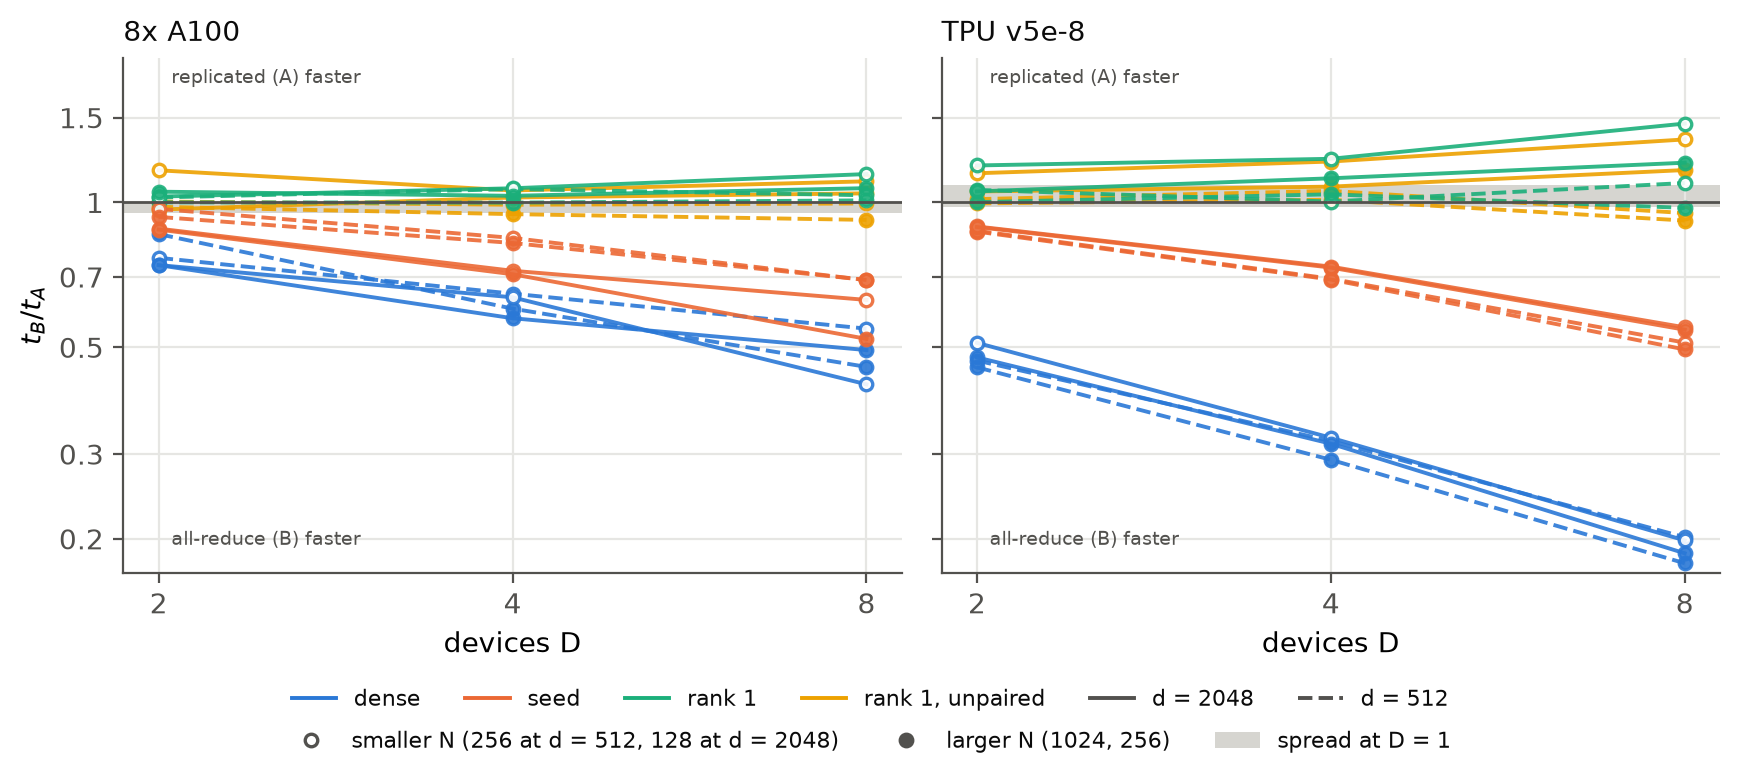
\includegraphics[width=0.88\textwidth]{f2b-crossover-vs-d.png}
  \caption{Split-update time divided by replicated-update time on the block benchmark.
    Below 1, splitting is faster; above 1, replication is faster. Panels separate hardware
    and matrix width. Marker shape identifies population size. Bars show the range from
    fastest split / slowest replicated repeat to slowest split / fastest replicated
    repeat, across five repeats per placement; these are not confidence intervals.
    The three main variants measured on both platforms are shown; the complete grids,
    including pairing variants, are in Appendix~\ref{sec:grids}.}
  \label{fig:f2}
\end{figure*}

At eight devices in one host, splitting the update is faster for every full-rank
configuration. For the dense and seed variants drawn in Figure~\ref{fig:f2}, the speedup
is 1.45--5.62$\times$. Dense alone gains 1.8--2.4$\times$ on the A100 and
5.0--5.6$\times$ on the v5e, so this result does not depend on the slower seed-regeneration
evaluation path. Replication is faster for rank-1 perturbations at width 2048
(Figure~\ref{fig:f2}). For those low-rank configurations, splitting takes 4--15\% longer
on the A100 and 17--46\% longer on the v5e. These low-rank ranges include both mirrored (drawn) and
unpaired sampling; Appendix~\ref{sec:grids} gives all variants and absolute times.

At width 512 the rank-1 placements are close. We treat a comparison as unresolved when
its repeat range contains 1, using the range defined in the figure caption. At eight
devices this occurs in six of the eight low-rank configurations at width 512. Every
full-rank configuration and every low-rank configuration at width 2048 has a repeat
range entirely on one side of 1. These repeats measure variation within a compiled run,
not variation across hardware sessions.

% generated by experiments/phase2/paper_evidence.py; do not edit
\begin{table*}[t]
\centering
\small
\caption{Worked example of Eq.~\ref{eq:crossover}, at width 2048, population 256 and eight devices. All times are milliseconds. $C_A$ and $C_B$ are separately measured reconstruction costs; $T_{\mathrm{add}}$ is communication added to the split reconstruction probe. The prediction is $C_A-C_B+T_{\mathrm{ag}}-T_{\mathrm{add}}$, including the small weight gather. Positive differences favor splitting. $t_A$ gives the generation time against which a penalty is divided in Figure~\ref{fig:f2}.}
\label{tab:worked}
\begin{tabular}{llrrrrrr}
\toprule
platform & variant & $C_A$ & $C_B$ & $T_{\mathrm{add}}$ & predicted $t_A-t_B$ & measured $t_A-t_B$ & $t_A$ \\
\midrule
A100 & seed & 61.05 & 7.78 & 1.25 & 52.03 & 54.30 & 113.26 \\
A100 & rank 1 & 0.77 & 0.35 & 1.62 & -1.19 & -1.40 & 19.88 \\
v5e & seed & 233.29 & 29.51 & 2.03 & 201.75 & 213.30 & 467.58 \\
v5e & rank 1 & 0.55 & 0.33 & 2.36 & -2.14 & -2.04 & 9.73 \\
\bottomrule
\end{tabular}
\end{table*}


Table~\ref{tab:worked} evaluates Eq.~\ref{eq:crossover} at one configuration on each
platform. Full-rank reconstruction costs 61--233\,ms, so splitting it easily pays for
1--2\,ms of communication. Rank-1 reconstruction costs less than 1\,ms; the communication
is then more expensive than the work saved. On the A100, the model gives a 1.19\,ms
penalty for splitting rank 1, against 1.40\,ms measured. On the v5e the measured penalty
is 2.04\,ms on a shorter replicated generation: 9.73\,ms against 19.88\,ms on the A100.
That makes the relative penalties 21\% and 7\% respectively.

The ratio plots and the timing equation describe the same difference:
$t_B/t_A=1-(t_A-t_B)/t_A$. Thus a fixed communication penalty can look larger as a ratio
when evaluation becomes faster. Table~\ref{tab:tb8} in the appendix reports the isolated communication
cost; Table~\ref{tab:worked} instead uses the cost added to a reconstruction probe,
which also includes any scheduling changes that operation causes.

\begin{figure*}[t]
  \centering
  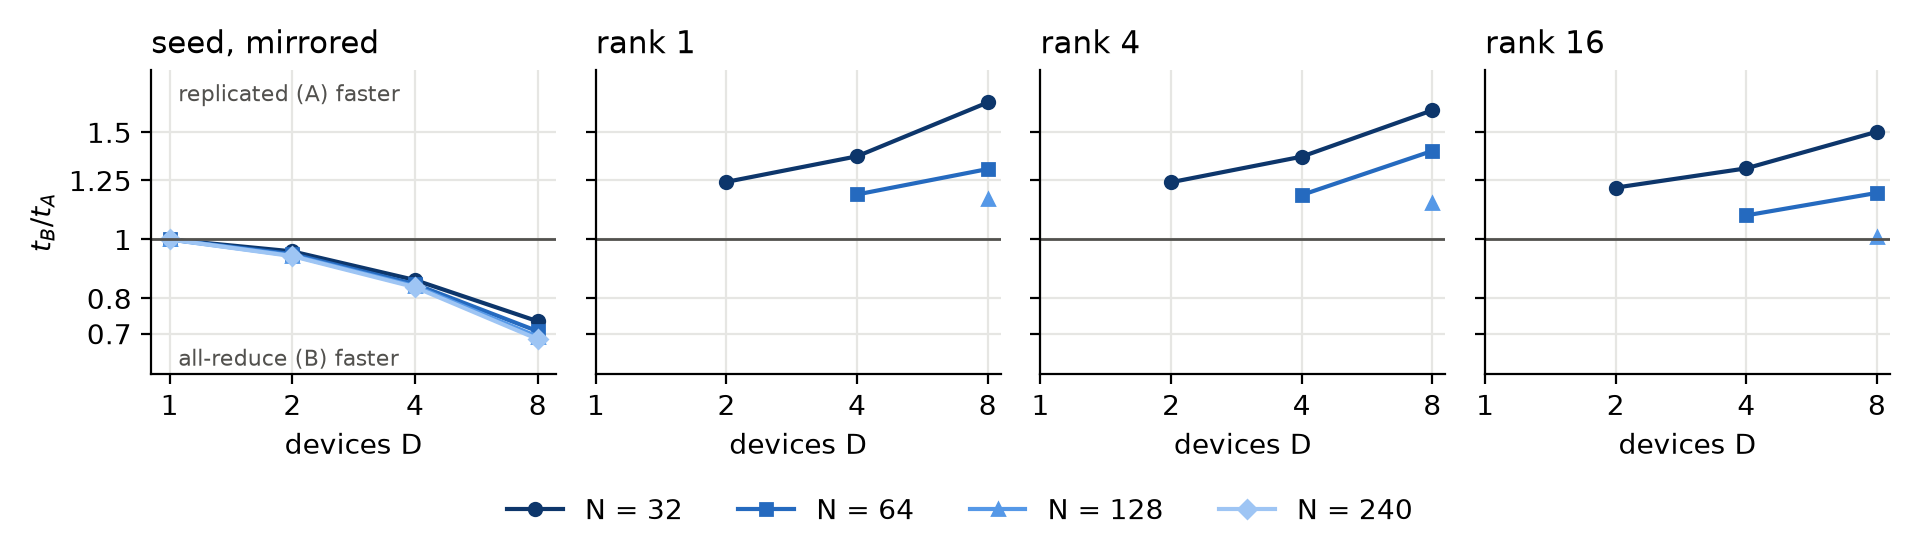
\includegraphics[width=\textwidth]{f9-e17-crossover.png}
  \caption{Placement on Qwen2.5-0.5B, TPU v5e: split / replicated time for a complete
    generation, including next-token loss evaluation. Splitting is faster for full-rank
    noise; replication is faster at every retained low-rank configuration. The strips
    below the plots distinguish fits, memory failures (OOM), and excluded comparisons.
    Only records stamped with a clean worktree are used; gaps are not connected.
    All one-device records are excluded. Absolute times are in Table~\ref{tab:tb5}.}
  \label{fig:f9}
\end{figure*}

Using separately measured reconstruction and added communication costs, the model
agrees with all 30 configurations whose repeat envelopes do not overlap. It agrees in
33 of 36 overall; its three misses are among the six near-ties. This is a check of whether
separately timed components account for complete generations, not a fit to their timing
differences. It was developed after the sweeps. Assuming ideal $1/D$ reconstruction and
using only the isolated collective benchmark misses two resolved A100 configurations.
Appendix~\ref{sec:timemodel} gives the comparison and the remaining errors in magnitude.

\subsection{Placement on a real model}



The same preference holds on Qwen2.5-0.5B on the TPU (Figure~\ref{fig:f9}).
We retain only records stamped with a clean worktree, leaving eight full-rank and twelve
low-rank timing comparisons. All eight-device records pass this filter.
Splitting helps full rank, with a larger advantage at eight than four devices.
Replication helps low rank; the rank-16, $N=128$ comparison is nearly tied, with a ratio
of 1.009 and a repeat envelope starting at 1.0006. Appendix~\ref{sec:memory} documents
the excluded records rather than treating them as missing because of memory limits.

The update contains 494,032,768 float32 values, including the tied embedding once:
1.84\,GiB. Scaling the isolated v5e communication time at 96\,MiB to this payload gives
39.4\,ms. This is an extrapolation of the measured communication rate, with no parameter
fit to Qwen's timing. The extra split cost for ranks 1 and 4 is 34--48\,ms in the
retained four- and eight-device comparisons. The payload estimate therefore explains
its scale, though it does not isolate the reconstruction contribution or test the
collective at this larger payload directly.

At eight devices, the rank-1 penalty stays roughly fixed as $N$ grows, while evaluation
time grows and the ratio approaches 1. Conversely, adding devices shortens evaluation,
so a nearly fixed penalty can produce a rising ratio. Rank 16 also reduces the absolute
penalty, to 2.4\,ms at $N=128$. The rank trend is not monotone: at $N=64$, rank 4 has a
ratio of 1.40, above rank 1's 1.31. The signs and a smaller rank-16 margin were expected
before this grid, after an earlier two-variant study; the population trend was observed
during the run.

At eight devices, all low-rank variants run out of memory at $N=240$, while full rank
fits. Low-rank evaluation batches candidates together; the full-rank variant regenerates
and evaluates them one at a time. This trades activation and weight memory against
throughput. Reduced-model compilation probes support the activation-memory explanation
(Appendix~\ref{sec:memory}); they do not establish an identical memory boundary on Qwen
with matched batching. Each placement comparison keeps batching fixed, whereas a timing
comparison across perturbation types includes this evaluation difference.

\subsection{Across a slow connection between hosts}
\label{subsec:boundary}

% generated by experiments/phase2/multihost/tb7_e18.py --latex; do not edit
\begin{table*}[t]
\centering
\small
\caption{The placement across a host boundary: $t_B - t_A$ in ms, negative where all-reduce (B) wins. Two 8$\times$A100 nodes joined by TCP sockets (InfiniBand carried no NCCL traffic); \texttt{1x8} is one node at $D{=}8$, \texttt{2x4} the same eight devices split across the boundary, \texttt{2x8} sixteen devices across it. The all-reduce runs at 64\,GiB/s on NVLink and 0.82 (\texttt{2x4}) and 0.58\,GiB/s (\texttt{2x8}) across the boundary. \emph{prereg.}: the prediction committed before the \texttt{2x8} configurations ran, whose bandwidth was $D$ times too high (the calibration all-reduced $1/D$ of its label). \emph{model} and \emph{corrected}: Eq.~\eqref{eq:crossover} on the same inputs with the bandwidth at the payload actually moved, computed after the measurements. The \texttt{1x8} column is re-measured on the cluster's first node; the model starts from the single-node sweep.}
\label{tab:tb7}
\begin{tabular}{llrrrrrrr}
\toprule
 & & & & \multicolumn{2}{c}{\texttt{2x4}} & \multicolumn{3}{c}{\texttt{2x8}} \\
\cmidrule(lr){5-6}\cmidrule(lr){7-9}
arm & $d$ & $N$ & \texttt{1x8} & measured & model & measured & prereg. & corrected \\
\midrule
seed & 2048 & 128 & $-21.4$ & $+86.8$ & $+91.0$ & $+74.1$ & $-13.9$ & $+137.2$ \\
seed & 2048 & 256 & $-50.8$ & $+57.2$ & $+58.7$ & $+56.7$ & $-48.2$ & $+103.0$ \\
seed & 512 & 1024 & $-20.1$ & $-13.0$ & $-18.9$ & $-24.8$ & $-27.0$ & $-17.6$ \\
rank 1 & 2048 & 128 & $+1.6$ & $+108.9$ & $+114.6$ & $+159.1$ & $+11.7$ & $+162.7$ \\
rank 1 & 2048 & 256 & $+1.4$ & $+111.4$ & $+114.4$ & $+130.9$ & $+11.4$ & $+162.5$ \\
rank 1 & 512 & 1024 & $0.0$ & $+6.9$ & $+7.1$ & $+7.8$ & $+0.8$ & $+10.2$ \\
\bottomrule
\end{tabular}
\end{table*}


Communication can reverse the full-rank preference. We repeated six configurations on
two A100 nodes. NCCL could not use the provider's InfiniBand, so cross-host traffic
ran over TCP sockets. The calibrated effective cross-host all-reduce bandwidth was
0.6--0.8\,GiB/s.

Keeping eight devices but splitting them between hosts adds 107--110\,ms to the
split placement's relative cost at width 2048 (Table~\ref{tab:tb7}). This exceeds the
21--51\,ms it saved on one host, so replication becomes faster for regenerated full-rank
noise. At width 512, the update is only 6\,MiB and splitting remains faster for that
variant. Replication's advantage for rank 1 grows across the slow connection.

The rule also gives a useful threshold for another connection. Keeping eight devices
and neglecting latency, the 96\,MiB all-reduce stops paying below about 4.1\,GiB/s at
$N=128$ and 1.8\,GiB/s at $N=256$. These are effective all-reduce rates, not network
line rates. They use the within-host savings plus the within-host communication being
replaced; Appendix~\ref{sec:boundary-audit} gives the calculation and repeat bounds.

Our prediction fixed before the sixteen-device run identified four of six faster
placements. Its bandwidth calibration used an incorrectly labelled message size.
Correcting that error after the runs gives all six preferences, but still overestimates
the split penalty by up to 63\,ms. The original prediction and the
retrospective correction remain side by side in Table~\ref{tab:tb7-audit}.
This experiment establishes the effect of a slow connection, not the performance of a
high-bandwidth multi-host cluster.

\subsection{What low-rank perturbations save}

\begin{figure*}[t]
  \centering
  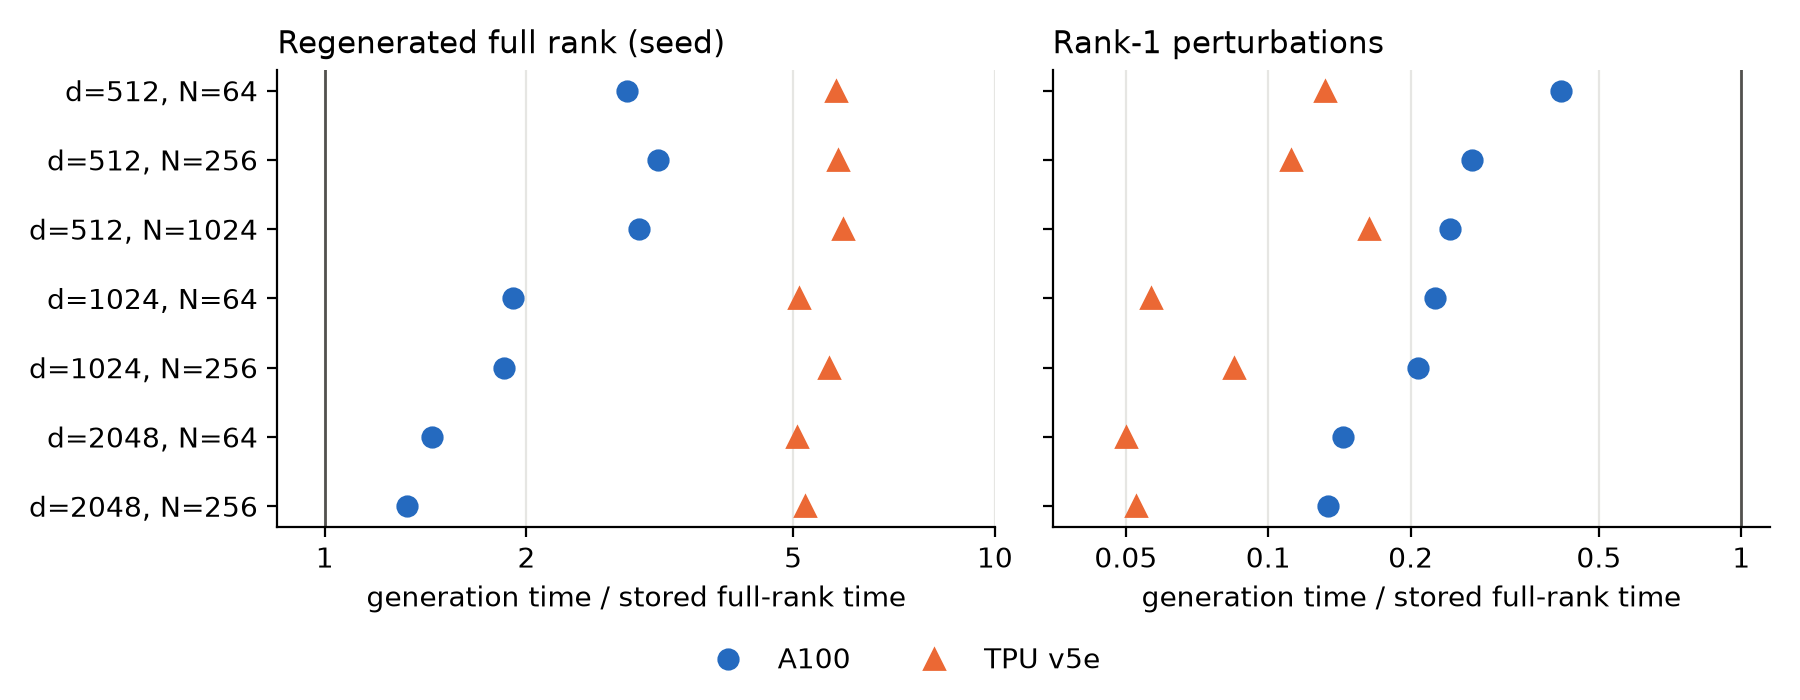
\includegraphics[width=0.9\textwidth]{f4-cost-common-bfloat16.png}
  \caption{Generation time relative to stored full-rank noise (dense), on one device
    with bfloat16 storage and default matrix-multiplication precision. Every row uses
    the same model width and population on both platforms, and all compared variants fit.
    Values below 1 are faster than dense. Low-rank noise has a larger relative advantage
    on the v5e at every common configuration. The full grid, including memory limits,
    is in Figure~\ref{fig:f4-full}.}
  \label{fig:f4}
\end{figure*}

On the simplified block, low-rank noise saves more relative to dense noise on the TPU
than on the GPU (Figure~\ref{fig:f4}). Across the same seven feasible configurations,
% generated by experiments/phase2/tb3.py; do not edit
rank-1 generation time is 0.22 times the dense time on the A100 and 0.08 times on the v5e (geometric means).

Regenerating full-rank noise instead trades speed for memory: the seed variant is slower
than dense at every comparable configuration, but fits the complete cost grid.
The full grid and precision comparisons are in Appendix~\ref{sec:systems-ablations}.
The platform difference persists at matched precision: the single-device scaling sweeps
use float32 storage and highest precision on both platforms, and give rank-1/dense time
geometric-mean ratios of 0.43 on A100 and 0.17 on v5e over seven matched
configuration/placement pairs.
These ratios describe the tested workload and implementation; they do not isolate the
hardware mechanism responsible for the difference.

As an implementation check, the library's single-device rank-1 throughput is within 3\% of
EGGROLL's released code on the A100, and 0.68--0.85 times its throughput on the v5e.
The TPU gap was not isolated. Appendix~\ref{sec:refimpl} separates these matched-device
comparisons from the additional throughput available with eight devices.

% CLAIM: at equal population the cheap perturbation aligns with the descent direction
% about as well, and on Countdown it ends at the same accuracy, with full rank ahead early.
% Evidence: tb6_e16.py (E15, E16), phase0/plot.py (E1), plot_e13.py and plot_e19.py
% (E13, E19).
\section{Is the cheaper update as good?}
\label{sec:quality}

A faster update is only worth having if it points in a useful direction. We compare the
perturbations at the same population, on the same loss, two ways: the alignment of one
update with the gradient-descent direction of a differentiable loss, and training on a
task scored by a non-differentiable reward.

\subsection{Alignment with the descent direction}

% F7 -- experiments/countdown/figures/f7-e13-heldout.png (plot_e13.py)
\begin{figure*}[t]
  \centering
  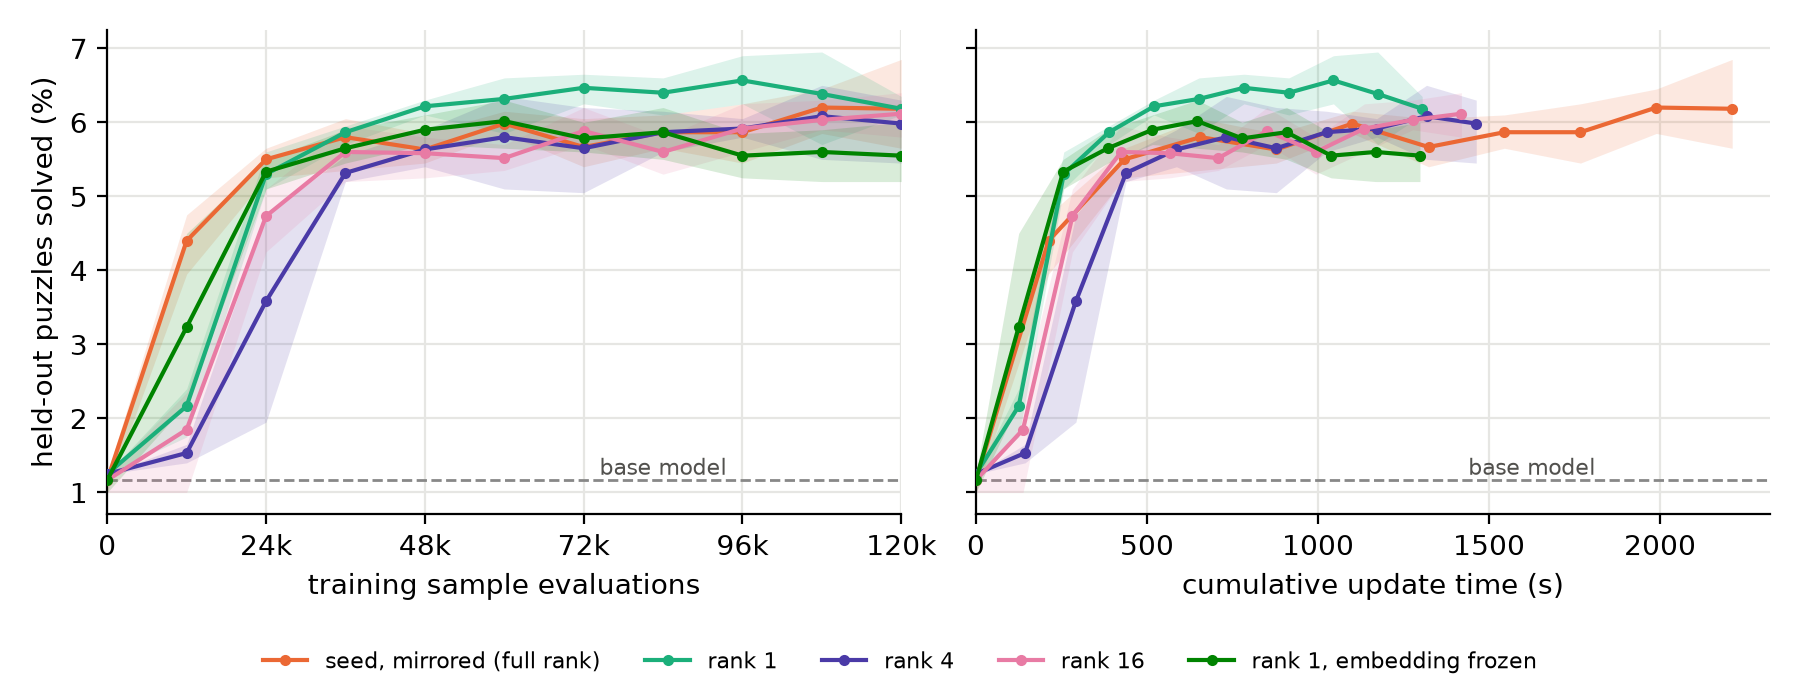
\includegraphics[width=0.84\textwidth]{f7-e13-heldout.png}
  \caption{Countdown with Qwen2.5-0.5B: the share of 2000 held-out puzzles solved,
    against scored training completions (left; 240 per update) and against cumulative
    update time (right), mean over three seeds with a min--max band. The time axis is
    each run's own seconds per update, as each arm was configured, without the first two
    updates (which compile) and without held-out decoding. At 12k samples full rank
    solves 4.4\% against 1.5--2.2\% for ranks 1, 4 and 16, with no overlap between
    seeds; every arm ends near 6\%.}
  \label{fig:f7}
\end{figure*}

We measure alignment as $\cos(\Delta\theta, -\nabla L)$, the cosine between one ES
update and the negative gradient of the next-token loss of Section~\ref{sec:setup}, on
Qwen2.5-0.5B with five perturbation seeds per configuration, and repeat two
configurations on a second prompt batch and on Qwen2.5-1.5B (Table~\ref{tab:tb6}). At
equal population the rank barely matters: rank 1 aligns 0.92--0.98 times as well as full
rank at both model sizes and on both batches, rank 16 0.97--1.05, and rank 4 1.04--1.31
(the 1.31 is at $N{=}30$, where five seeds spread widely: full rank measures 1.3--1.9
and rank 4 0.7--2.0, Table~\ref{tab:tb6-audit}). Unpaired rank 1 is 1.36$\times$
mirrored rank 1 at $N{=}240$, close to the $\sqrt2$ that $N$ against $N/2$ directions
gives, and 1.17$\times$ at $N{=}30$; mirroring halves the directions and in exchange
halves the stored factors.

% generated by experiments/countdown/tb6_e16.py --latex; do not edit
\begin{table}[t]
\centering
\small
\setlength{\tabcolsep}{3.2pt}
\caption{Cosine between one ES update and the exact gradient of the
  next-token loss ($\times 10^{-4}$, median over 5 perturbation seeds), at equal
  population; \emph{1 unp.} is rank 1 without mirrored pairs.
  \emph{ref.}: the mirrored full-rank fit from the synthetic block
  (Figure~\ref{fig:f5}) at the same $N/P$, a post hoc reference; unpaired
  sampling should sit about $\sqrt2$ above it. Batch 2 repeats two
  configurations on freshly drawn prompts. Ranges and the preregistered
  predictions are in Table~\ref{tab:tb6-audit}.}
\label{tab:tb6}
\begin{tabular}{lrrrrrrr}
\toprule
 & & \multicolumn{5}{c}{rank} & \\
\cmidrule(lr){3-7}
model & $N$ & full & 1 & 4 & 16 & 1 unp. & ref. \\
\midrule
0.5B & 30 & $1.42$ & $1.37$ & $1.87$ & $1.49$ & $1.60$ & $1.56$ \\
0.5B & 240 & $4.23$ & $3.91$ & $4.42$ & $4.09$ & $5.33$ & $4.48$ \\
0.5B, batch 2 & 240 & $4.20$ & $3.91$ & -- & -- & -- & $4.48$ \\
1.5B & 30 & $0.83$ & $0.77$ & -- & -- & -- & $0.87$ \\
1.5B & 240 & $2.32$ & $2.27$ & -- & -- & -- & $2.51$ \\
\bottomrule
\end{tabular}
\end{table}


The cosines are of order $10^{-4}$, and that is expected. A Gaussian-projection
approximation predicts alignment proportional to $\sqrt{N/P}$: $\sqrt{3/\pi}\,\sqrt{N/P}$
for unpaired sampling and $1/\sqrt2$ of that for mirrored pairs, and with $P$ = 494M and
$N$ = 30, $\sqrt{N/P}$ is $2.5\times10^{-4}$. The approximation closely describes the
synthetic block, where every arm is within 0.91--1.02 of it at every rank
(Figure~\ref{fig:f5}), and the mirrored arms here measure 0.80--0.92 of it (1.10 for
rank 4 at $N{=}30$). Its applicability to low-rank perturbations depends on the
gradient's structure (Appendix~\ref{sec:alignment}). Most of each update is not along the
descent direction.

The predictions we committed before these runs overestimated low-rank alignment: the
measurements came out at 0.43--0.67 of the prediction at 0.5B, and 23--26\% below it at
1.5B even after a correction fixed in advance. They read each arm's synthetic fit against a
different variable. The $N/P$ reading used here, and Table~\ref{tab:tb6}'s reference
column, were developed afterward; Appendix~\ref{sec:alignment} gives both predictions and
why the first missed.

\subsection{Training on a task}

We trained on Countdown, arithmetic puzzles in the style of TinyZero \citep{tinyzero2025},
with settings adapted from \citet{qiu2025}: their population of 30, noise scale
$\sigma{=}10^{-3}$ and learning rate, converted to Eq.~\ref{eq:update}; centered ranks
where they standardize rewards (the weights' standard deviation is 0.29 against 1, and
we did not match the resulting update magnitudes); and 8 puzzles per update where their
protocol uses 200 samples
(Appendix~\ref{sec:countdown} has the full setup). Each arm runs 500 updates, 120,000
scored training completions, with three seeds, on one A100. A completion scores 1 if it
solves the puzzle and 0.1 if it is well formed but wrong. Held-out accuracy is measured
on 2000 disjoint puzzles by greedy decoding every 50 updates.

The base model solves 1.2\% of the held-out puzzles and formats 43\% of its answers.
Formatting is learned at once: every arm formats 98.5\% or more by the first evaluation,
so Figure~\ref{fig:f7} shows the solve rate, which carries everything that differs
between arms. Training raises it to a plateau, 6.0--6.2\% for full rank and ranks 1, 4
and 16 at the end, and 5.55\% with the embedding frozen (27\% of the parameters). The
approach differs. At the first evaluation, 12k samples in, full rank solves 4.4\% of the
puzzles and ranks 1, 4 and 16 solve 1.5--2.2\%, with the seed ranges apart; by 36k
samples every arm is at 5.3--5.9\%. With one evaluation on the rising part of the curve
we can say that full rank learns faster per sample early on, not by how much.

Per update, rank 1 is faster. As configured, a steady-state update took 4.44\,s at full
rank and 2.62\,s at rank 1, 1.69$\times$. Part of that is how the two arms evaluate: the
full-rank arm scored its members in chunks of five, and the low-rank arm scores the whole
population in one batch. With both batching every member, on one host, the times are
3.62\,s and 2.52\,s: rank 1 updates 1.44$\times$ faster for the same evaluation. Against
update time (Figure~\ref{fig:f7}, right) the early gap mostly closes: full rank solves
4.4\% after 212\,s of updates and 5.5\% after 434\,s, rank 1 5.3\% after 257\,s. The
evaluations are too sparse to say which reaches a given solve rate first, and that axis
uses the arms as configured, not with matched batching.

The task separates training from failure, not small differences in update quality. A
population-16 run, fixed in advance as a positive control because by the square-root scaling
it aligns 27\% worse per update, does not test that either: on about the same budget it
takes 940 updates (120,320 completions) to population 30's 500 and reaches the plateau
sooner (Figure~\ref{fig:f7c}). Among the runs that update all parameters, no rank breaks
training or ends at a different accuracy, on one task at one model size with three
seeds; the run with the embedding frozen ends lower.

% CLAIM: none of ours.
\section{Related work}
\label{sec:related}

\paragraph{ES at scale.} \citet{salimans2017} made distributed ES practical by sending
scalar returns rather than gradients; ARS \citep{mania2018} and deep neuroevolution
\citep{such2017,conti2017,chrabaszcz2018} share its simple design. \citet{qiu2025} and
EGGROLL \citep{eggroll2025} carry it to language models from opposite sides, exact noise
regenerated from seeds and cheap low-rank noise. \citet{cho2026reward} show that reward
design and normalization change how large a population must be, which is independent of
where the sum is computed. Neither \citet{qiu2025} nor EGGROLL compares update
placements, or both designs in one implementation on GPUs and TPUs.

\paragraph{Zeroth-order optimization for language models.} MeZO \citep{malladi2023} also
estimates gradients from forward passes, with the goal of training in inference-sized
memory rather than evaluating a population in parallel. It is a close relative with a
different bottleneck.

\paragraph{Estimators.} Gaussian-smoothing and zeroth-order analyses make the dependence
on dimension explicit \citep{nesterov2017,duchi2015,berahas2022}. Natural ES, CMA-ES and
information-geometric optimization adapt richer search distributions
\citep{wierstra2014,hansen2001,hansen2016,ollivier2017}; we hold the optimizer fixed and
vary the perturbation. Structured orthogonal and coupled Monte Carlo samples promise gains
from designing perturbations jointly \citep{choromanski2018structured,rowland2018coupled};
on our synthetic block, orthogonal Hadamard and scrambled Sobol sampling gave none
(Appendix~\ref{sec:alignment}), a result about this high-dimensional, small-population
regime only.

\paragraph{Distributed systems.} JAX and GSPMD provide the compiler and sharding we build
on \citep{jax2018,gspmd2021}. evosax \citep{lange2022evosax} is the standard JAX ES
library; its dense population matrix is the memory ceiling in Table~\ref{tab:tb1}.
\citet{sheng2020tpu} run distributed ES on TPUs for meta-learning, without comparing
placements or accelerators. ZeRO \citep{rajbhandari2020zero} shards optimizer state and
gradients in data-parallel training, the same trade between replicated work and
communicated bytes that separates our two placements.

\section{Conclusion}

Exchanging only scalar scores can make distributed ES repeat substantial work.
Splitting update reconstruction helps when the computation saved exceeds the cost of
communicating a model-sized update. In our single-host measurements, this favors
splitting for full-rank perturbations and replication for low-rank perturbations at
large matrix width. The same preference holds on Qwen2.5-0.5B on the TPU. Across the
measured slow connection between A100 hosts, large full-rank updates favor replication too.

To choose a placement, measure reconstruction and the added communication cost in the
relevant computation context. Isolated communication benchmarks and ideal $1/D$ compute
scaling can misestimate the small differences that decide low-rank cases. The model
explains most measured preferences but is not an exact decision rule.

Low-rank perturbations also reduce generation time relative to stored full-rank noise
on the block, especially on the tested TPU. Their updates have similar measured
directional alignment, and the tested ranks reach similar observed final Countdown
accuracy. Full rank learns faster per sample at the first checkpoint. The limited
learning experiments support using the cheaper perturbations in this setting, while
leaving broader learning-efficiency comparisons open.


\ifanonymous\else
\section*{Acknowledgements}
The TPU measurements ran on Kaggle's free TPU v5e-8 tier; the GPU measurements ran on
rented A100 nodes. No grant or employer resources were used.
\fi

\bibliographystyle{plainnat}
\bibliography{references}

\appendix

\section{Measurement details}
\label{sec:implementation}

\paragraph{Repeatability.} With fitness scores held fixed, one- and eight-device
Qwen2.5-0.5B updates agree to $6.3\times10^{-6}$ relative error in the norm of the whole parameter tree on the A100. The committed log reports this aggregate; it does not bound every leaf. Two
20-generation runs of the same eight-device program agree byte for byte. Separately
compiled programs need not follow the same training trajectory: changes in floating-point
arithmetic can change the selected token when greedy-decoding logits are nearly tied.

\subsection{The cost of ranking}
\label{sec:barrier}

Centered ranks require the scores of all candidates. Each device gathers and sorts
the same list. In an isolated v5e benchmark over 84 configurations, the ranking step
takes at most 60\,$\mu$s for populations up to a thousand and about 0.2\,ms at 4096.
At $N=2^{18}$, sorting takes 12.1\,ms and does not become faster with more devices,
because every device repeats it. Going from one to eight devices adds 9--10\,$\mu$s
at populations up to a thousand and 38.5\,$\mu$s at $N=2^{18}$. The isolated 1\,MiB score gather costs about 20\,$\mu$s, accounting for roughly half of the latter increase.
In full generations, turning score shaping on adds 41\,$\mu$s at $d=512$, $N=1024$
and 149\,$\mu$s at $d=2048$, $N=256$, within the repeat spread. Very large populations
should therefore budget for sorting even when gathering the scores is cheap.

\subsection{How the timing components are measured}
\label{sec:timemodel}

% generated by experiments/phase2/tb8.py; do not edit by hand
\begin{table}[t]
\centering
\small
\setlength{\tabcolsep}{4pt}
\caption{What one more collective costs inside a running program ($\mu$s; the slope of a dependent chain), $D{=}8$. The rows are what the placements issue: B's all-reduce of the $4P$-byte update and the $4N$-byte fitness gather. A program holding only the collective also pays a one-op floor (0.32\,ms on the A100, 0.60\,ms on the v5e) that a generation pays once. $\beta$ is payload over time.}
\label{tab:tb8}
\begin{tabular}{llrr}
\toprule
collective & payload & A100 & v5e \\
\midrule
all-reduce, latency floor & 8\,B & 27.2 & 5.7 \\
all-reduce (B), $d{=}512$ & 6\,MiB & 117.3 & 122.5 \\
all-reduce (B), $d{=}2048$ & 96\,MiB & 925.2 & 2006.0 \\
fitness gather, $N{=}256$ & 1\,KiB & 8.1 & 3.8 \\
fitness gather, $N{=}1024$ & 4\,KiB & 8.0 & 5.0 \\
fitness gather, $N{=}262144$ & 1\,MiB & 20.7 & 19.8 \\
\midrule
$\alpha$ ($\mu$s) & & 27 & 6 \\
$\beta$ (GiB/s) & & 98 & 47 \\
\bottomrule
\end{tabular}
\end{table}


Table~\ref{tab:tb8} uses a communication-only probe with a dependent chain of operations.
The increase in run time per additional operation estimates the collective's marginal
cost, excluding the fixed launch and synchronization cost of the compiled call. That
fixed cost is 0.32\,ms on the A100 and 0.60\,ms on the v5e. These are isolated
communication measurements, not timings extracted from a training trace.

\texttt{contraction\_isolation.py} similarly times three reconstruction probes: the
replicated path, the split path with its all-reduce, and the local split computation
with the all-reduce removed. The last two give $C_B$ and an estimate of the added cost
of communication. That difference can include scheduling changes caused by the
collective. It is not a directly isolated kernel duration.

The recorded replicated-probe slope includes A's gather of rank-derived weights.
\texttt{timemodel.py} subtracts the separately measured gather to obtain $C_A$ before
applying Eq.~\ref{eq:crossover}, so the gather is counted once.

Small reconstruction computations do not split ideally. On the A100,
$C_A/(D C_B)$ is 0.60--1.01 for full-rank noise and 0.18--0.45 for rank 1.
At width 2048, adding the all-reduce to the low-rank reconstruction probe costs
1.75--1.80 times the isolated communication benchmark on the A100, and 1.18--1.19 times
on the v5e. With measured local computation
and this added cost, the median absolute timing-model discrepancy is 0.63\,ms on the
A100 and 0.48\,ms on the v5e. The faster placement is identified in 18 of 20 and 15
of 16 configurations respectively; the three disagreements have measured gaps of
0.02--0.09\,ms. Correctly identifying a preference does not imply an accurate estimate
of its size: the largest discrepancies are 9.19\,ms on the A100 and 25.22\,ms on the
v5e. \texttt{timemodel.py} reports every configuration.

The measured-components model agrees with all 18 resolved A100 and all 12 resolved v5e
comparisons. The counts differ between platforms because the mirrored full-rank variant
was run only on A100. Replacing $C_B$ by $C_A/D$ and using the isolated collective
benchmark gives 17/20 and 16/16 sign agreements, including two resolved A100 misses:
mirrored rank 1 at $(d,N)=(512,256)$ and unpaired rank 1 at $(2048,256)$. For A100
low-rank noise at width 2048, this simple model predicts $t_A-t_B$ between $-0.49$
and $+0.18$\,ms, against $-1.63$ to $-0.84$\,ms measured. Keeping ideal splitting but
using the communication added to the reconstruction probe improves the counts to 19/20
and 16/16. Thus measured local reconstruction does not improve every near-tie; the added
communication cost is the important refinement for the resolved A100 cases.
\texttt{paper\_evidence.py} reproduces these comparisons and Table~\ref{tab:worked}.

\paragraph{What was fixed before measuring.} Before the single-host sweeps we expected
splitting to favor full-rank noise and replication to favor low-rank noise. The original
byte counts were subsequently corrected from compiled programs to include both score
and weight gathers. The timing equation was developed after these sweeps. It was used
prospectively at the host boundary, where the original prediction and the correction
below must be distinguished.

\subsection{Host-boundary prediction audit}
\label{sec:boundary-audit}

% generated by experiments/phase2/multihost/tb7_e18.py --latex; do not edit
\begin{table*}[t]
\centering
\small
\caption{Host-boundary prediction audit: split minus replicated time ($t_B-t_A$), in ms; negative favors splitting. Columns give hosts $\times$ devices per host. The original sixteen-device prediction used an overstated bandwidth; \emph{model} and \emph{corrected} use the actual calibration payload and were computed after the runs. Effective cross-host all-reduce bandwidth was 0.82\,GiB/s at eight devices and 0.58\,GiB/s at sixteen devices. The model starts from the earlier single-host sweep; the measured \texttt{1x8} column is a new measurement on the cluster's first host.}
\label{tab:tb7-audit}
\begin{tabular}{llrrrrrrr}
\toprule
 & & & & \multicolumn{2}{c}{\texttt{2x4}} & \multicolumn{3}{c}{\texttt{2x8}} \\
\cmidrule(lr){5-6}\cmidrule(lr){7-9}
variant & $d$ & $N$ & \texttt{1x8} & measured & model & measured & original & corrected \\
\midrule
seed & 2048 & 128 & $-21.4$ & $+86.8$ & $+91.0$ & $+74.1$ & $-13.9$ & $+137.2$ \\
seed & 2048 & 256 & $-50.8$ & $+57.2$ & $+58.7$ & $+56.7$ & $-48.2$ & $+103.0$ \\
seed & 512 & 1024 & $-20.1$ & $-13.0$ & $-18.9$ & $-24.8$ & $-27.0$ & $-17.6$ \\
rank 1 & 2048 & 128 & $+1.6$ & $+108.9$ & $+114.6$ & $+159.1$ & $+11.7$ & $+162.7$ \\
rank 1 & 2048 & 256 & $+1.4$ & $+111.4$ & $+114.4$ & $+130.9$ & $+11.4$ & $+162.5$ \\
rank 1 & 512 & 1024 & $0.0$ & $+6.9$ & $+7.1$ & $+7.8$ & $+0.8$ & $+10.2$ \\
\bottomrule
\end{tabular}
\end{table*}


The calibration used for the sixteen-device prediction all-reduced $1/D$ of its labelled
payload, overstating bandwidth by a factor of $D$. This was discovered after the runs.
Table~\ref{tab:tb7-audit} retains the prediction made with that calibration and the
retrospective correction at the actual payload size. The latter identifies all six
preferences, but overestimates the split penalty by up to 63\,ms. The calibration
and isolated ladder use different payloads and timing methods; their bandwidth numbers
are not evidence of a difference between hardware sessions.

For the fixed-eight-device comparison, let $S=t_A-t_B$ be the within-host saving and
$T_{\mathrm{intra}}$ the communication being replaced. Neglecting latency and holding
reconstruction costs fixed, the cross-host break-even rate is
$\beta_*=4P/(S+T_{\mathrm{intra}})$. At width 2048, $S$ is 21.4 or 50.8\,ms at
$N=128$ or 256; the within-host bandwidth term at 96\,MiB is 1.46\,ms. This gives
4.1 and 1.8\,GiB/s. Using repeat extremes gives 2.9--4.2 and 1.5--2.1\,GiB/s.
These are approximate effective collective rates, including algorithmic traffic in the
measured bandwidth, not line rates. The earlier sixteen-device prediction had the same
ordering, with thresholds of 4.12 and 1.70\,GB/s (decimal units); it also assumed extra
compute savings from using sixteen devices. The two calculations are not identical tests.

\paragraph{Other placements and overlap.} The two placements are not exhaustive.
One primary device can reconstruct the whole update and broadcast the model, as in
EGGROLL's vLLM setup \citep[Appendix L.2]{eggroll2025}. It avoids repeated reconstruction
across replicas, but retains a full reconstruction on the critical path and adds a
model-sized broadcast. We did not benchmark this third placement. Under an otherwise
identical synchronous cost model it adds communication to A; heterogeneous devices,
memory limits and implementation differences could change the comparison. Hierarchical
or compressed communication also changes the tradeoff; PowerSGD communicates low-rank
approximations of updates rather than the dense arrays studied here \citep{vogels2019}.
Overlapping an update's all-reduce with the next generation's evaluation would use stale
weights. Within a generation, bucketing partial updates could overlap local reconstruction with
communication, as in distributed backpropagation \citep{li2020ddp}. Such overlap can
at best replace $C_B+T_{\mathrm{ar}}$ by $\max(C_B,T_{\mathrm{ar}})$ under the
accounting model. With the measured probe costs, replication retains a 0.40--1.98\,ms
lead at every low-rank width-2048 configuration. This is a conditional bound from
\texttt{overlap\_bound.py}, not an implemented overlap experiment.



\subsection{What model size alone can predict}
\label{sec:size}

A conditional scaling argument helps separate parameter count from implementation
constants. Suppose the leading low-rank reconstruction cost is $C_A=kPNr$, with $k$ absorbing
pairing and arithmetic efficiency, and $C_B=qC_A$. Write the collective time
as $\alpha+4P/\beta$. Equation~\ref{eq:crossover} then favors splitting when
\[
  (1-q)kNr > \frac{4}{\beta}
               +\frac{\alpha-T_{\mathrm{ag}}(4N)}{P}.
\]
For bandwidth-dominated communication, fixed $k,q,\beta$ and large $P$, the leading
parameter-count dependence cancels. Population times rank, rather than parameter count
alone, then sets the balance. For full-rank noise, the analogous assumption is
$C_A=kPN$. These assumptions are not automatic: matrix shapes and compiler fusion change
$k$, small local computations change $q$, and the collective rate depends on message size
and topology. Factor generation also has terms proportional to $Nr(m+n)$ rather than
$P$. We therefore do not turn the block's constants into a universal threshold or a
claim about 7B models. Such a model would need to fit on each device, and its
reconstruction and collective costs would need measurement.

\section{Cost and implementation comparisons}
\label{sec:systems-ablations}
\label{sec:refimpl}

\begin{figure*}[t]
  \centering
  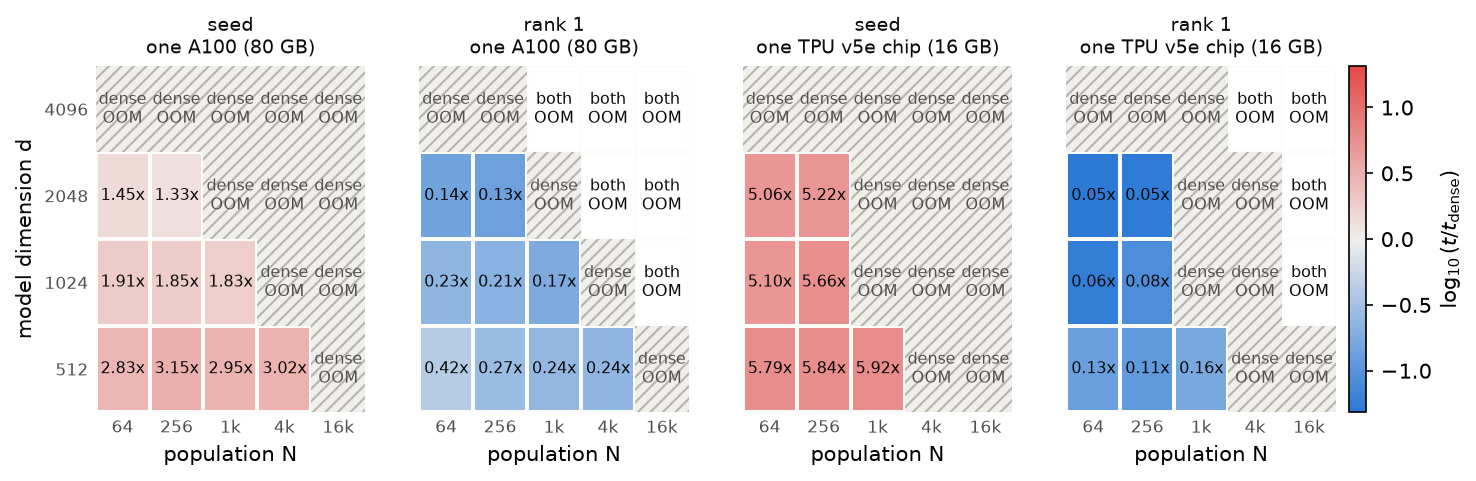
\includegraphics[width=\textwidth]{f4-cost-bfloat16.png}
  \caption{The full single-device cost and feasibility grid, relative to stored
    full-rank noise at each model width and population. Blue is faster, red slower.
    Hatched cells mean the dense baseline does not fit; blank cells marked ``both OOM''
    mean neither variant fits. Memory feasibility is separate from a measured speedup.
    The main text compares only configurations feasible on both platforms.}
  \label{fig:f4-full}
\end{figure*}

% generated by experiments/phase2/tb3.py; do not edit by hand
\begin{table*}
\centering
\small
\caption{Systems ablations, assembled from committed results. Each ratio is the time of the first variant over the second (below one: the first is faster), as a geometric mean over the configurations where both were measured (n: how many).}
\label{tab:tb3}
\begin{tabular}{p{0.30\linewidth}p{0.22\linewidth}p{0.40\linewidth}}
\toprule
ablation & where & result \\
\midrule
cost, rank 1 vs dense & A100, bf16 & 0.22x (n=9) \\
cost, rank 4 vs dense & A100, bf16 & 0.27x (n=9) \\
cost, rank 16 vs dense & A100, bf16 & 0.29x (n=9) \\
cost, rank 1 vs dense & TPU v5e, bf16 & 0.08x (n=7) \\
cost, rank 4 vs dense & TPU v5e, bf16 & 0.09x (n=7) \\
cost, rank 16 vs dense & TPU v5e, bf16 & 0.11x (n=7) \\
cost, bf16 vs f32 & A100, dense & 1.12x (n=8) \\
cost, bf16 vs f32 & A100, seed & 1.08x (n=20) \\
cost, bf16 vs f32 & A100, rank 1 & 1.00x (n=14) \\
cost, bf16 vs f32 & TPU v5e, dense & 0.93x (n=6) \\
cost, bf16 vs f32 & TPU v5e, seed & 1.01x (n=20) \\
cost, bf16 vs f32 & TPU v5e, rank 1 & 0.97x (n=16) \\
cost, highest vs default & TPU v5e, dense & 1.08x (n=5) \\
cost, highest vs default & TPU v5e, rank 1 & 1.85x (n=6) \\
cost, highest vs default & TPU v5e, rank 16 & 1.64x (n=6) \\
cost, highest vs default & TPU v5e, rank 4 & 1.76x (n=6) \\
cost, highest vs default & TPU v5e, seed, mirrored & 1.02x (n=6) \\
cost, highest vs default & TPU v5e, seed & 1.02x (n=6) \\
\bottomrule
\end{tabular}
\end{table*}


Figure~\ref{fig:f4-full} includes the configurations excluded from the common-grid speed
comparison because one or more variants do not fit. Table~\ref{tab:tb3} separates three
choices: perturbation rank, storage datatype, and matrix-multiplication precision.
The precision setting controls internal multiplication accuracy, separately from array
storage. On the v5e, forcing JAX's highest precision instead of its default costs the
low-rank variants 1.6--1.9 times in run time and the full-rank variants at most 8\%.
Its effect on learning accuracy was not measured. Default precision reduces low-rank
reconstruction cost further, which, with communication fixed, favors replication in
Eq.~\ref{eq:crossover}; the placement sweeps nevertheless keep highest precision fixed. Storage datatype alone changes the
reported geometric-mean times by much less; it should not be confused with this
precision setting.

% generated by experiments/phase2/tb1.py; do not edit by hand
\begin{table*}[t]
\centering
\small
\setlength{\tabcolsep}{5pt}
\caption{Throughput at matched shapes: token-position evaluations per second (tokens = population $\times$ batch $\times$ sequence). \emph{rank 1} and \emph{seed} are this library's variants; \emph{EGGROLL} is its authors' released code; \emph{naive} gives every member its own copy of the weights, evaluating the population in parallel; \emph{evosax} is OpenES in the incumbent JAX library. None of the three references shards, so only the library's variants have a $D{=}8$ column. Seed evaluates one candidate at a time to keep weight memory at $O(P)$. Qiu et al.'s released code is not included. OOM: does not fit the device at this shape.}
\label{tab:tb1}
\begin{tabular}{llrrrrrrr}
\toprule
 & & \multicolumn{2}{c}{rank 1} & EGGROLL & \multicolumn{2}{c}{seed} & naive & evosax \\
\cmidrule(lr){3-4}\cmidrule(lr){6-7}
shape & platform & $D{=}1$ & $D{=}8$ & $D{=}1$ & $D{=}1$ & $D{=}8$ & $D{=}1$ & $D{=}1$ \\
\midrule
$d{=}512$, $N{=}256$ & A100 & 21.30M & 27.24M & 21.76M & 1.43M & 5.86M & 5.19M & 5.36M \\
$d{=}512$, $N{=}256$ & TPU v5e & 23.33M & 46.80M & 27.29M & 484k & 3.54M & 3.71M & 2.97M \\
$d{=}512$, $N{=}1024$ & A100 & 26.03M & 84.46M & 25.56M & 1.45M & 9.44M & 5.42M & 5.58M \\
$d{=}512$, $N{=}1024$ & TPU v5e & 16.77M & 149.67M & 24.72M & 486k & 3.81M & 3.74M & 2.33M \\
$d{=}2048$, $N{=}128$ & A100 & 2.97M & 6.79M & 3.05M & 314k & 1.87M & 406k & 375k \\
$d{=}2048$, $N{=}128$ & TPU v5e & 3.35M & 7.02M & 4.15M & 34k & 266k & 204k & OOM \\
$d{=}2048$, $N{=}256$ & A100 & 3.20M & 10.88M & 3.21M & 315k & 2.06M & 409k & 377k \\
$d{=}2048$, $N{=}256$ & TPU v5e & 3.22M & 13.03M & 4.52M & 34k & 270k & 140k & OOM \\
\bottomrule
\end{tabular}
\end{table*}


\paragraph{Matched-device comparison.} Table~\ref{tab:tb1} compares released
implementations at the same block configurations. The naive baseline gives each
candidate a separate copy of the model; evosax uses OpenES. At one device, the library's
rank-1 throughput is 0.97--1.02 times EGGROLL's on the A100 and 0.68--0.85 times on
the v5e. The TPU difference was not isolated. We did not benchmark Qiu et al.'s released
implementation, so the seed column is not a timing of their code.

\paragraph{Additional devices.} The tested reference implementations do not split the
population across devices. The eight-device columns therefore show extra throughput
from extra hardware, not equal-resource speedups over those references. Compared with
one-device EGGROLL, the library on eight devices reaches 1.3--3.4 times the throughput on A100
and 1.7--6.1 times on v5e. The full scaling grids report each implementation path against
its own smallest device count.

\paragraph{Implementation boundaries.} EGGROLL's reference rank-1 path does not compile
on a 16\,GB TPU chip at $d=512$, $N=16384$: it requests 24.1\,GiB of temporaries.
The library avoids this compiler behavior by padding rank-1 factors with a zero column
on TPU, retaining a fused multiply; it runs that configuration in 245\,ms. The GPU
compiler does not need the padding. The tested reference also declines embedding tables,
which the library supports through the same interface as matrix layers. These are properties
of the tested code versions, not limitations of the algorithms.


\section{Real-model timing and memory}
\label{sec:memory}

% generated by experiments/countdown/tb5_e17.py --latex; do not edit
\begin{table*}[t]
\centering
\small
\caption{What one real-model update costs, in ms (Qwen2.5-0.5B, one ask, next-token loss and tell on the fixed prompt batch, TPU v5e-8, median of five repeats). Each entry is the faster of the two placements; Figure~\ref{fig:f9} gives the ratio between them. OOM: neither placement fits a 16\,GB chip at that shape.}
\label{tab:tb5}
\begin{tabular}{llrrrr}
\toprule
arm & $N$ & $D{=}1$ & $D{=}2$ & $D{=}4$ & $D{=}8$ \\
\midrule
seed, mirrored & 32 & 4902 & 2481 & 1263 & 673 \\
seed, mirrored & 64 & 9788 & 4893 & 2469 & 1276 \\
seed, mirrored & 128 & 19559 & 9718 & 4882 & 2482 \\
seed, mirrored & 240 & 36658 & 18159 & 9102 & 4590 \\
rank 1 & 32 & OOM & 217 & 109 & 71 \\
rank 1 & 64 & OOM & OOM & 219 & 122 \\
rank 1 & 128 & OOM & OOM & OOM & 230 \\
rank 1 & 240 & OOM & OOM & OOM & OOM \\
rank 4 & 32 & OOM & 211 & 111 & 72 \\
rank 4 & 64 & OOM & OOM & 214 & 119 \\
rank 4 & 128 & OOM & OOM & OOM & 227 \\
rank 4 & 240 & OOM & OOM & OOM & OOM \\
rank 16 & 32 & OOM & 225 & 117 & 78 \\
rank 16 & 64 & OOM & OOM & 241 & 136 \\
rank 16 & 128 & OOM & OOM & OOM & 272 \\
rank 16 & 240 & OOM & OOM & OOM & OOM \\
\bottomrule
\end{tabular}
\end{table*}


Table~\ref{tab:tb5} gives absolute generation times behind Figure~\ref{fig:f9}.
The original grid has 128 records; 63 carry a dirty-worktree flag. Historical launch
scripts ran other probes first, which could dirty result files, but no per-run diff
was saved to certify that only outputs changed. We therefore exclude those records.
The remaining 65 include 43 timings and 22 memory failures; only configurations with
two clean records enter a placement comparison. This leaves twelve low-rank and eight
full-rank timing comparisons. All eight-device records are clean. Excluded comparisons
are dashes, distinct from observed memory failures; historical records remain available
for audit in the experiment directory.

At eight devices, ranks 1, 4 and 16 fit populations up to 128 and all fail at 240; the
regenerated full-rank variant fits all four populations. The evaluation schedules differ:
full rank scans individual candidates, while low rank batches them with a shared base
weight matrix. A diagnostic CPU compilation probe on a reduced model finds temporary
memory growing with candidates and prompts when candidates are batched. Batching
full-rank evaluation in the same way reproduces that growth, rather than the flat
population dependence of scanning. This supports an activation-memory explanation,
but is not a measured matched-batching memory boundary for Qwen on TPU.

\section{Synthetic alignment}
\label{sec:alignment}

% generated by experiments/countdown/tb6_e16.py --latex; do not edit
\begin{table*}[t]
\centering
\small
\caption{Alignment measurements and prediction audit ($\times10^{-4}$; median [min, max] across five seeds). \emph{Later reference} uses the full-rank synthetic fit at $N/P$, selected after the runs. \emph{Original prediction} was fixed before each run and uses the variant's fit at $N/d_{\mathrm{samp}}$ (with the advance correction at 1.5B described in the text). Ratios are measured / predicted.}
\label{tab:tb6-audit}
\begin{tabular}{lllrrrrr}
\toprule
 & & & & \multicolumn{2}{c}{later reference} & \multicolumn{2}{c}{original prediction} \\
\cmidrule(lr){5-6}\cmidrule(lr){7-8}
model & arm & $N$ & measured & pred. & ratio & pred. & ratio \\
\midrule
0.5B & seed, mirrored & 30 & $1.42$ [1.3, 1.9] & $1.56$ & $0.91$ & $1.56$ & $0.91$ \\
0.5B & seed, mirrored & 240 & $4.23$ [3.8, 4.4] & $4.48$ & $0.94$ & $4.48$ & $0.94$ \\
0.5B & rank 1 & 30 & $1.37$ [1.2, 1.7] & $1.56$ & $0.88$ & $2.69$ & $0.51$ \\
0.5B & rank 1 & 240 & $3.91$ [3.8, 4.2] & $4.48$ & $0.87$ & $7.57$ & $0.52$ \\
0.5B & rank 4 & 30 & $1.87$ [0.7, 2.0] & $1.56$ & $1.20$ & $2.78$ & $0.67$ \\
0.5B & rank 4 & 240 & $4.42$ [4.1, 4.8] & $4.48$ & $0.99$ & $7.85$ & $0.56$ \\
0.5B & rank 16 & 30 & $1.49$ [1.1, 1.7] & $1.56$ & $0.95$ & -- & -- \\
0.5B & rank 16 & 240 & $4.09$ [3.9, 4.5] & $4.48$ & $0.91$ & -- & -- \\
0.5B & rank 1, unpaired & 30 & $1.60$ [1.1, 1.9] & $1.56$ & $1.03$ & $3.76$ & $0.43$ \\
0.5B & rank 1, unpaired & 240 & $5.33$ [5.1, 5.5] & $4.48$ & $1.19$ & $10.56$ & $0.50$ \\
\midrule
0.5B, second batch & seed, mirrored & 240 & $4.20$ [3.8, 4.4] & $4.48$ & $0.94$ & $4.48$ & $0.94$ \\
0.5B, second batch & rank 1 & 240 & $3.91$ [3.8, 4.2] & $4.48$ & $0.87$ & $7.57$ & $0.52$ \\
\midrule
1.5B & seed, mirrored & 30 & $0.83$ [0.8, 0.9] & $0.87$ & $0.95$ & $0.87$ & $0.95$ \\
1.5B & seed, mirrored & 240 & $2.32$ [2.0, 2.6] & $2.51$ & $0.92$ & $2.51$ & $0.92$ \\
1.5B & rank 1 & 30 & $0.77$ [0.4, 1.1] & $0.87$ & $0.89$ & $1.04$ & $0.74$ \\
1.5B & rank 1 & 240 & $2.27$ [1.9, 2.4] & $2.51$ & $0.91$ & $2.93$ & $0.77$ \\
\bottomrule
\end{tabular}
\end{table*}




% F5 -- experiments/phase0/figures/f5-estimator-quality.png (experiments/phase0/plot.py)
\begin{figure}[t]
  \centering
  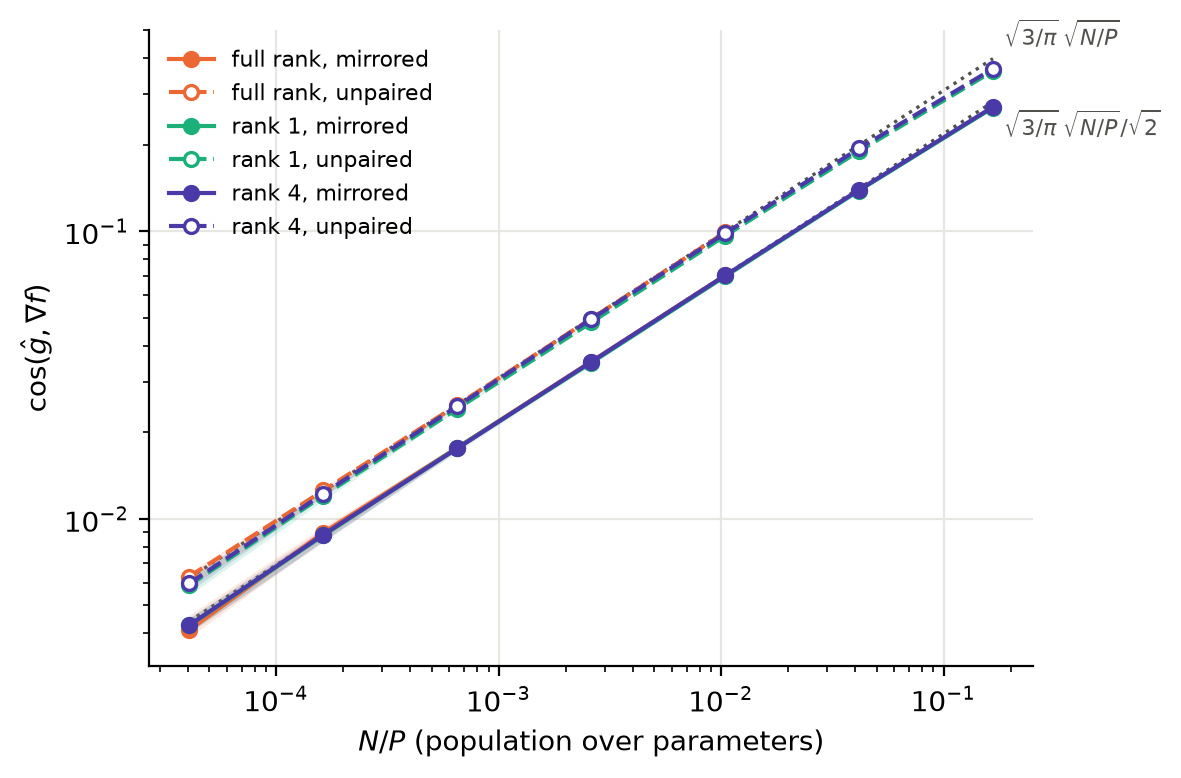
\includegraphics[width=\linewidth]{f5-estimator-quality.png}
  \caption{Alignment on the synthetic block ($\sigma{=}10^{-3}$, centered ranks):
    $\cos(\Delta\theta, -\nabla L)$ for the squared-error loss, against $N/P$, median and
    interquartile band over 30 replicates. The three ranks lie on top of each other.
    Dotted: the Gaussian-projection approximation, unpaired and mirrored.}
  \label{fig:f5}
\end{figure}

\paragraph{The Gaussian-projection approximation.} Let $z_i$ be member $i$'s
perturbation projected onto the unit descent direction, $\langle\epsilon_i, -\nabla
L\rangle/\lVert\nabla L\rVert$. It has unit variance for full-rank and for low-rank
noise, since $UV^\top/\sqrt r$ has identity covariance. If the loss is locally linear,
ranking the members by loss ranks them by $z_i$, and if $z_i$ is Gaussian each
$\epsilon_i$ enters Eq.~\ref{eq:update} with a coefficient close to $\Phi(z_i)-\tfrac12$
for large $N$. The update's component along the
descent direction is then about $N\,\mathbb{E}[(\Phi(z)-\tfrac12)\,z] = N/(2\sqrt\pi)$
and, for $N\ll P$, its norm is about $\sqrt{NP\,\mathbb{E}[(\Phi(z)-\tfrac12)^2]} =
\sqrt{NP/12}$, so the cosine is $\sqrt{3/\pi}\,\sqrt{N/P}$. A mirrored pair contributes
one direction with twice the weight, and $N/2$ of them give $1/\sqrt2$ of that.

\paragraph{When the projection is Gaussian.} For full-rank Gaussian noise $z_i$ is
exactly Gaussian. For rank-$r$ noise on a matrix with gradient $G$, the projection is a
sum over the $r$ factor pairs of $a^\top G b$, summed again over matrices. If $G$ has
rank one, $G = uv^\top$, each term is $(a^\top u)(v^\top b)$, a product of two Gaussians,
however many entries of $G$ are nonzero. The projection approaches a Gaussian as the
gradient spreads over many singular directions and many matrices, and as $r$ grows. We
did not measure the gradient's spectrum on Qwen, so for the real model the approximation
is a scale estimate, not a derivation.

Figure~\ref{fig:f5} is the synthetic study behind Section~\ref{sec:quality}, one slice
of 456 configurations of 30 replicates each. Against $N/P$ the mirrored variants of every
rank coincide, the largest over the smallest at equal $N$ being 1.01--1.04, and every
variant is within 0.91--1.02 of the approximation; its log-log slopes are 0.494--0.508. Unpaired sampling lies 1.34--1.53$\times$ above mirrored, about $\sqrt2$.
Orthogonal (Hadamard) and scrambled Sobol sampling, not drawn, are within 0.97--1.04 of
plain mirroring. That null result holds for this high-dimensional, small-population
regime; it is not a claim about coupled sampling in general.

The predictions frozen before the real-model runs used $N/d_{\mathrm{samp}}$ instead,
where $d_{\mathrm{samp}}$ is the number of independent random numbers in one
perturbation: the parameter count for full-rank noise and $r(m+n)$ per $m\times n$
matrix at rank $r$ (other parameters count fully). Each variant's own fit against that axis
was the prediction, and Table~\ref{tab:tb6-audit} keeps it next to the synthetic reference. Its extra 0.5B
prompt check reuses the same perturbation keys and changes only puzzle numbers within
the same prompt template. It measures sensitivity to that change, not an independent
replication; it is excluded from the main table. On the block, where every matrix is $512\times512$, $P/d_{\mathrm{samp}}$ is
256 at rank 1 and 64 at rank 4. On Qwen2.5 the matrices are larger and not square, and it
is 638 and 171 at 0.5B and 1063 and 287 at 1.5B, so the same $N$ sits further right on
the $N/d_{\mathrm{samp}}$ axis than on the block and the fitted curve predicts higher alignment. At a
slope of one half that overstates rank 1 by $\sqrt{638/256}\approx1.6$ and rank 4 by
$\sqrt{171/64}\approx1.6$ at 0.5B, against measured shortfalls of 1.9--2.0 and 1.5--1.8.
The same fits predicted full rank within 9\%, since $P/d_{\mathrm{samp}}$ is 1 for it on
every model. For rank 1 at 1.5B the prediction was multiplied by a correction of 0.53
measured at 0.5B and fixed in advance; the observations were still 23--26\% below it.


At equal population, unpaired rank 1 has 1.36 times the mirrored alignment at $N=240$
and 1.17 times at $N=30$ on the original 0.5B batch. The former is close to the
$\sqrt2$ ratio of the independent-direction approximation. This comparison is specific
to the tested loss and noise scale; it does not establish that unpaired sampling is
better for training. The theoretical approximation and the fitted synthetic reference
are also distinct: the latter is the reference column in Table~\ref{tab:tb6-audit}.


\section{Countdown details}
\label{sec:countdown}

\begin{table*}[t]
\centering
\small
\caption{Countdown training configuration. A sample evaluation is one scored \emph{training}
  completion (held-out scoring is not counted); every population-30 variant uses 240 per update (30
  members $\times$ 8 puzzles), so 120,000 is 500 updates.}
\label{tab:e2e}
\begin{tabular}{lp{0.76\linewidth}}
\toprule
task, reward & Countdown; 1.0 solved, 0.1 well formed but wrong, 0.0 otherwise \\
data & training pool of 256 puzzles, 8 per update; 2000 disjoint held-out puzzles \\
prompts, decoding & chat template, prompts padded to 128 tokens, 96 new tokens; greedy \\
variants & $N{=}30$, $\sigma{=}10^{-3}$, $\eta{=}5\times10^{-7}$ in Eq.~\ref{eq:update},
  centered ranks; seed, mirrored and ranks 1, 4, 16, plus rank 1 with the embedding (27\%
  of the parameters) frozen \\
budget, seeds & 120,000 sample evaluations per run; seeds 0--2 per variant \\
evaluation & 2000 held-out puzzles every 50 updates, before the first and after the last \\
hardware & one A100-SXM4-80GB; about 13\,h for the campaign \\
\bottomrule
\end{tabular}
\end{table*}

\paragraph{Relation to the published setup.} \citet{qiu2025} use
$\Delta\theta=\alpha\sum_i z_i\epsilon_i/N$ with $\alpha=5\times10^{-4}$ and
standardized rewards $z_i$. Taking $\eta=\alpha\sigma$ converts their learning-rate
convention to Eq.~\ref{eq:update}. Our centered ranks replace standardized rewards;
the nominal weight standard deviations are about 0.29 and 1, and we did not match the
resulting update magnitudes. Our batches contain eight puzzles per update rather than
200 samples. The experiment therefore compares our perturbation variants, not a
reproduction of the published learning curve.

\paragraph{Timing.} The time axis in Figure~\ref{fig:f7} excludes updates 0 and 1,
which compile (322--635\,s each), and all held-out decoding. These are material costs
for a short run; the axis is steady-state update time rather than total experiment time.
The displayed learning curves use the campaign with clean recorded provenance.
Diagnostic batching probes are not used as reported performance results.

\begin{figure}[t]
  \centering
  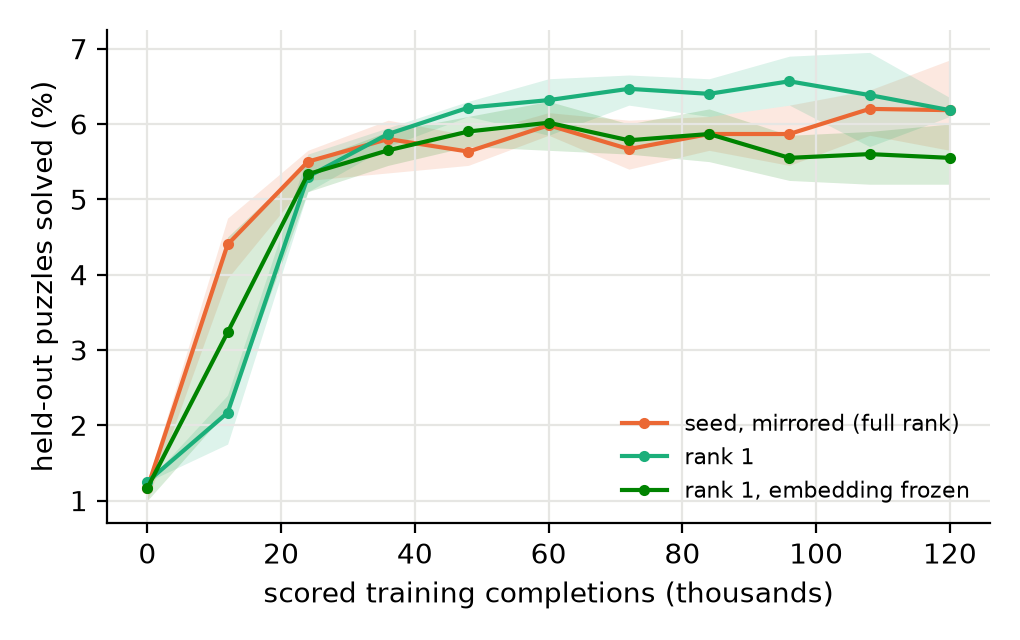
\includegraphics[width=\linewidth]{f7-e13-frozen.png}
  \caption{Freezing the embedding changes which parameters can train. The frozen
    embedding accounts for 27\% of parameters; this rank-1 variant ends at a lower
    observed solve rate. Means and min--max bands over three seeds.}
  \label{fig:f7-frozen}
\end{figure}

\paragraph{Freezing the embedding.} This variant asks what leaving the tied embedding
out of training costs. It contains 27\% of the parameters, and the tested EGGROLL
reference declines it (Appendix~\ref{sec:refimpl}). The library can perturb it without
forming a full table per candidate. Freezing it gives 5.55\% mean final solve rate
[5.20, 6.00], against 6.18\% [6.10, 6.35] for rank 1 updating all parameters, with
non-overlapping seed ranges (Figure~\ref{fig:f7-frozen}). Thus embedding support has
value in this experiment, although this extra intervention is not a comparison of
perturbation ranks alone.

\begin{figure}[t]
  \centering
  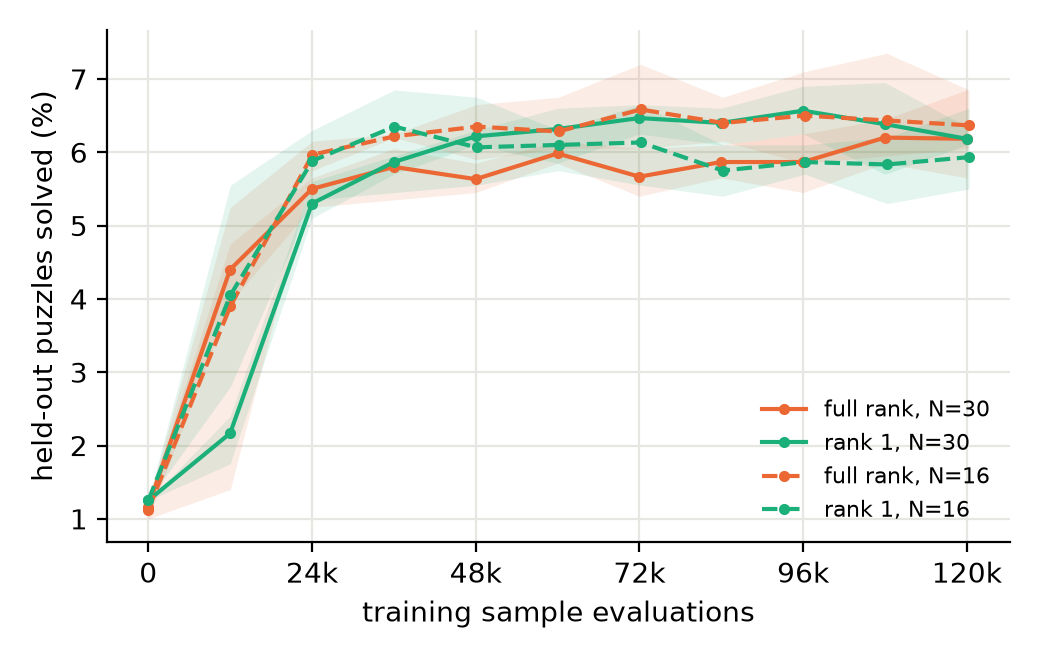
\includegraphics[width=\linewidth]{f7c-e19-n16.png}
  \caption{An additional population-size experiment: population 30 (solid, 500 updates)
    and 16 (dashed, 940 updates), with about 120,000 scored completions each and three
    seeds per variant. Population 16 approaches the plateau sooner per completion, but
    also receives more updates. This does not isolate per-update alignment.}
  \label{fig:f7c}
\end{figure}

\paragraph{The intended positive control.} The population-16 run was fixed in advance
as a control with 27\% lower predicted per-update alignment. At approximately the same
completion budget it takes 940 updates instead of 500 and reaches the plateau sooner
(Figure~\ref{fig:f7c}). Thus it does not establish that this task can distinguish small
differences in update quality. The final observed accuracy is similar.

\section{Scaling grids}
\label{sec:grids}

Figures~\ref{fig:m1-a100}--\ref{fig:m2-tpu} are the full strong- and weak-scaling grids,
every perturbation variant under both placements. Both show parallel efficiency, each series against its
own smallest measured device count, so the ideal is 1 for every series; the strong-scaling
figures add time per generation, and the weak-scaling figures peak memory per device. At $d{=}2048$ and 32 members per device the rank-1 variants keep
0.86--0.93 efficiency at eight devices on the A100 and 0.71--0.91 on the v5e. What
degrades is a placement: under replication the dense and seed variants fall to 0.39 and 0.50
on the A100 (0.18 and 0.54 on the v5e), because they have the most work to repeat, and
under all-reduce the same variants hold 0.79--1.00. The v5e grid has efficiencies above one,
all at $d{=}512$ (rank 1 at $N{=}1024$ reaches 1.22 at $D{=}2$): there the single chip is
memory-bound, and splitting the population relieves it. The dense variant with all-reduce has
no one-device point at $d{=}2048$, $N{=}256$ on the v5e (out of memory), so its efficiency
is normalized at $D{=}2$.

% M1/M2 per platform. Explicit paths: the A100 and TPU sets share filenames.
\begin{figure*}[p]
  \centering
  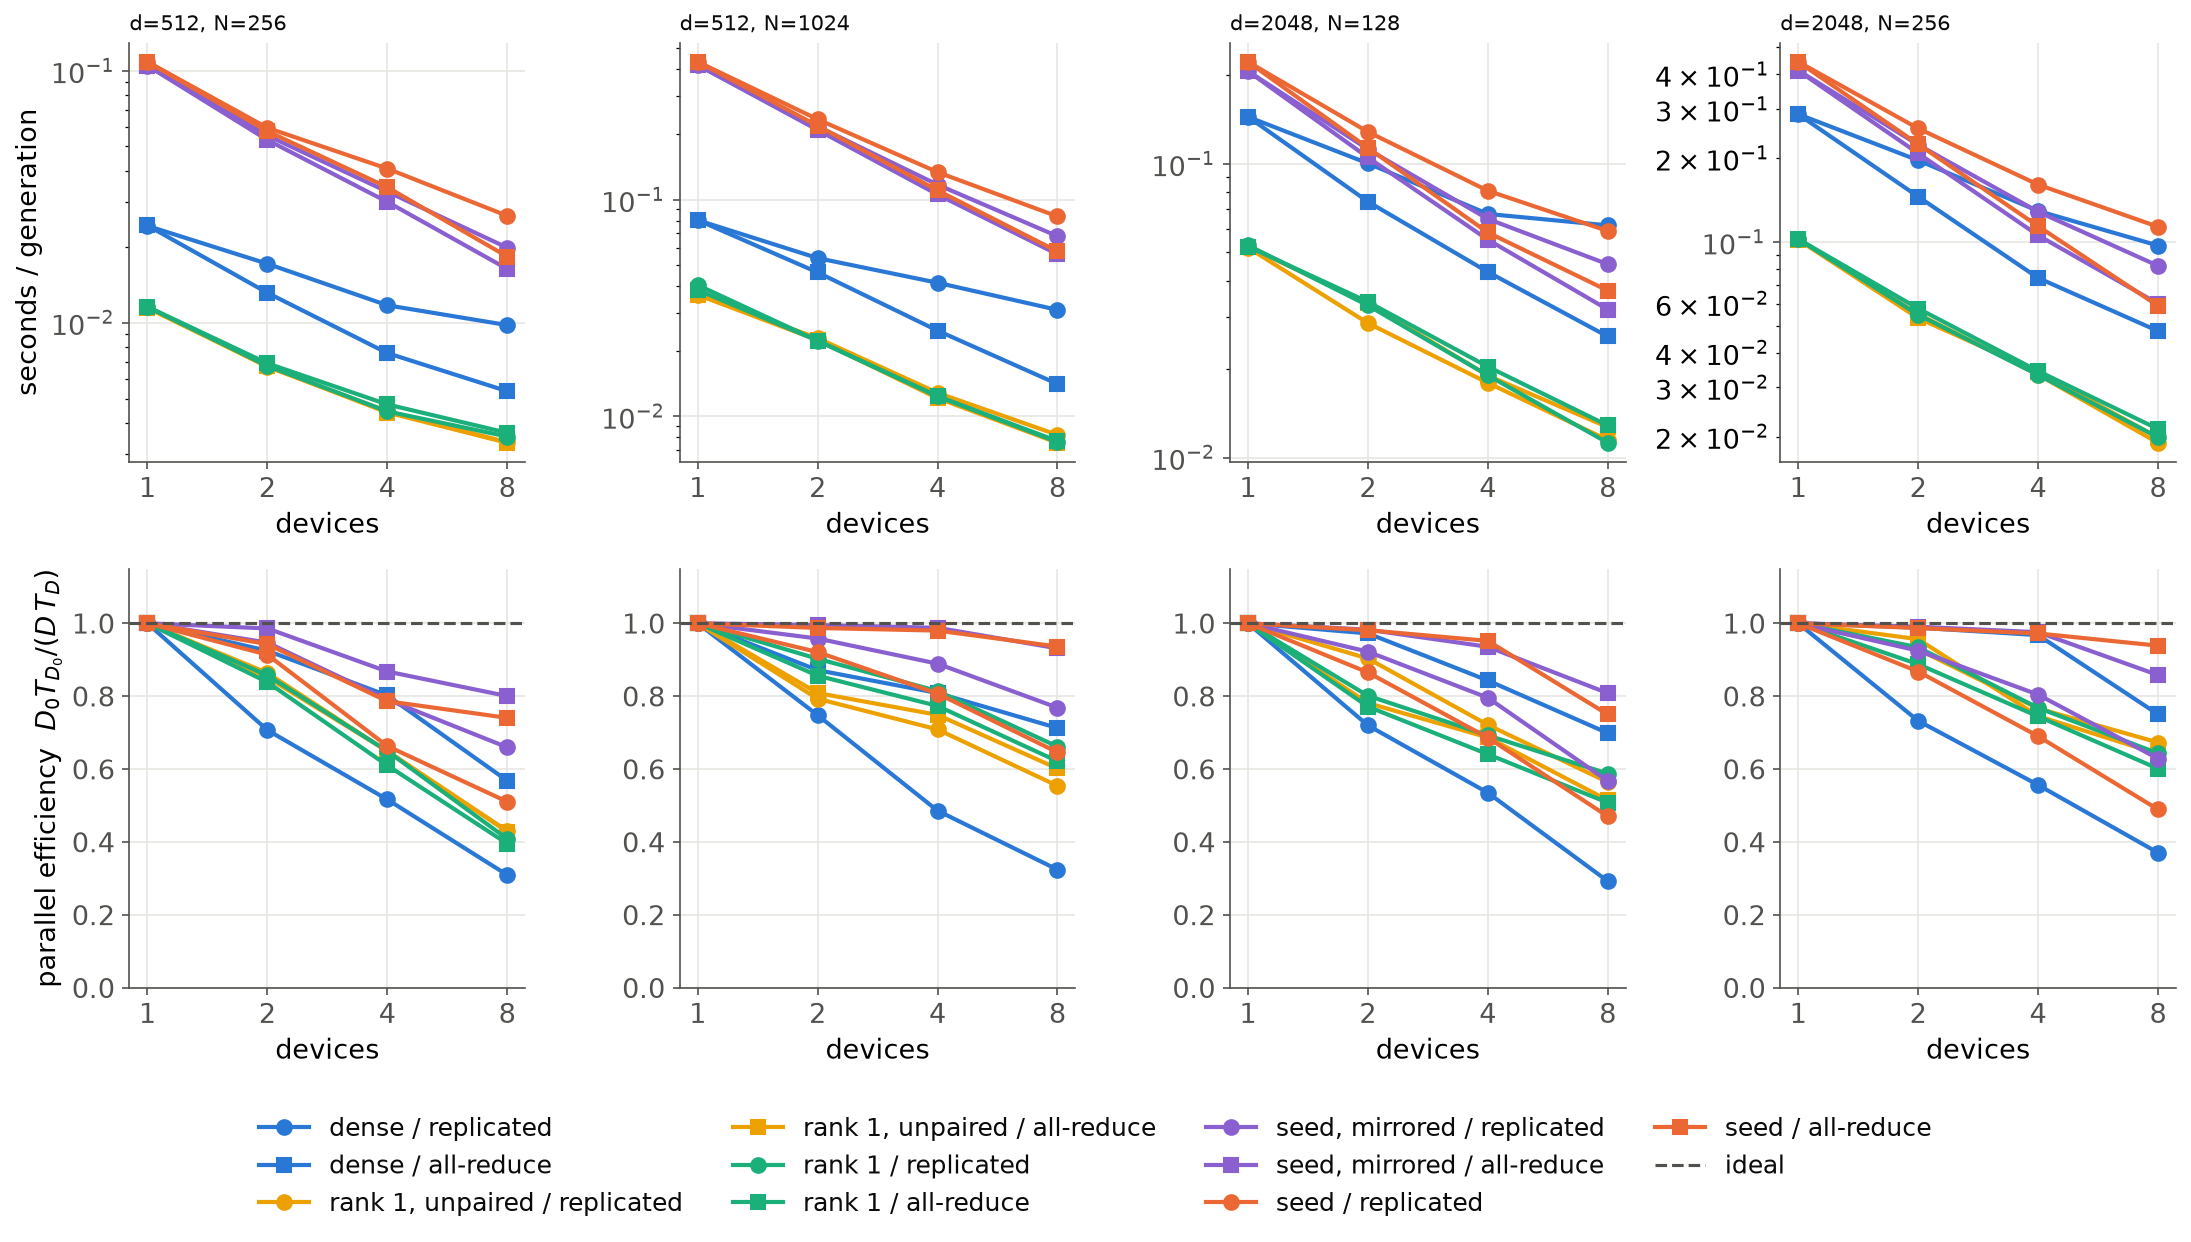
\includegraphics[width=.9\textwidth]{../experiments/phase2/figures/m1-strong-scaling.png}
  \caption{A100 strong scaling at fixed total population: generation time (top) and
    parallel efficiency (bottom), relative to each series' smallest device count.
    An efficiency of 1 means ideal scaling. Every perturbation variant is shown under
    both replicated and split update placement.}
  \label{fig:m1-a100}
\end{figure*}
\begin{figure*}[p]
  \centering
  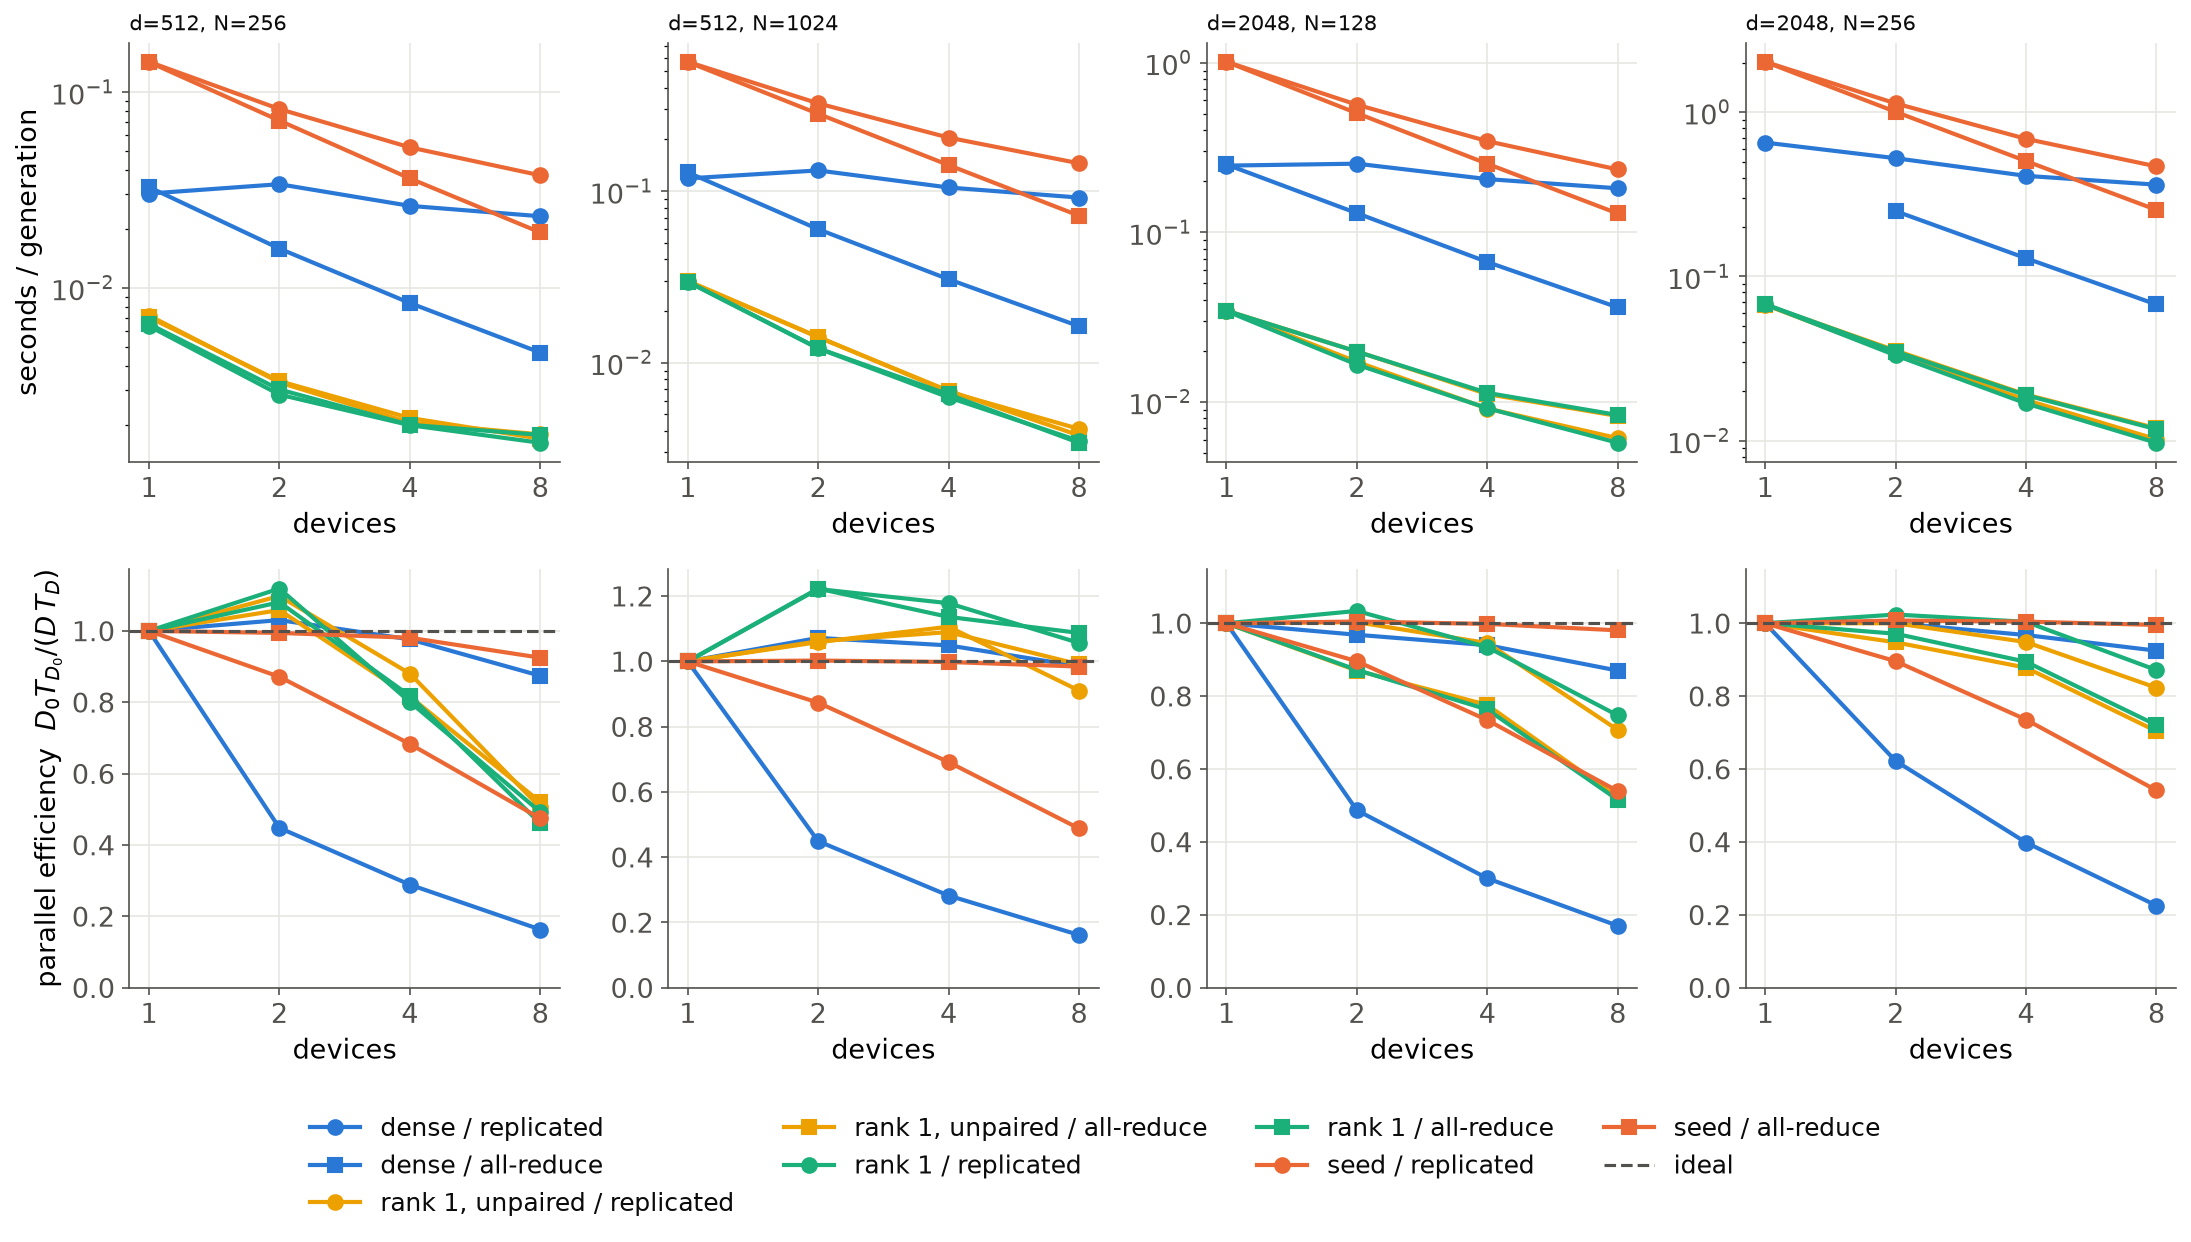
\includegraphics[width=.9\textwidth]{../experiments/phase2/figures-tpu-v5e8/m1-strong-scaling.png}
  \caption{TPU strong scaling at fixed total population: generation time (top) and
    efficiency (bottom). Dense noise with splitting at $d=2048$, $N=256$ is normalized
    at two devices because it does not fit on one. Some width-512 cases exceed unit
    efficiency when splitting the population relieves the single-device bottleneck.}
  \label{fig:m1-tpu}
\end{figure*}
\begin{figure*}[p]
  \centering
  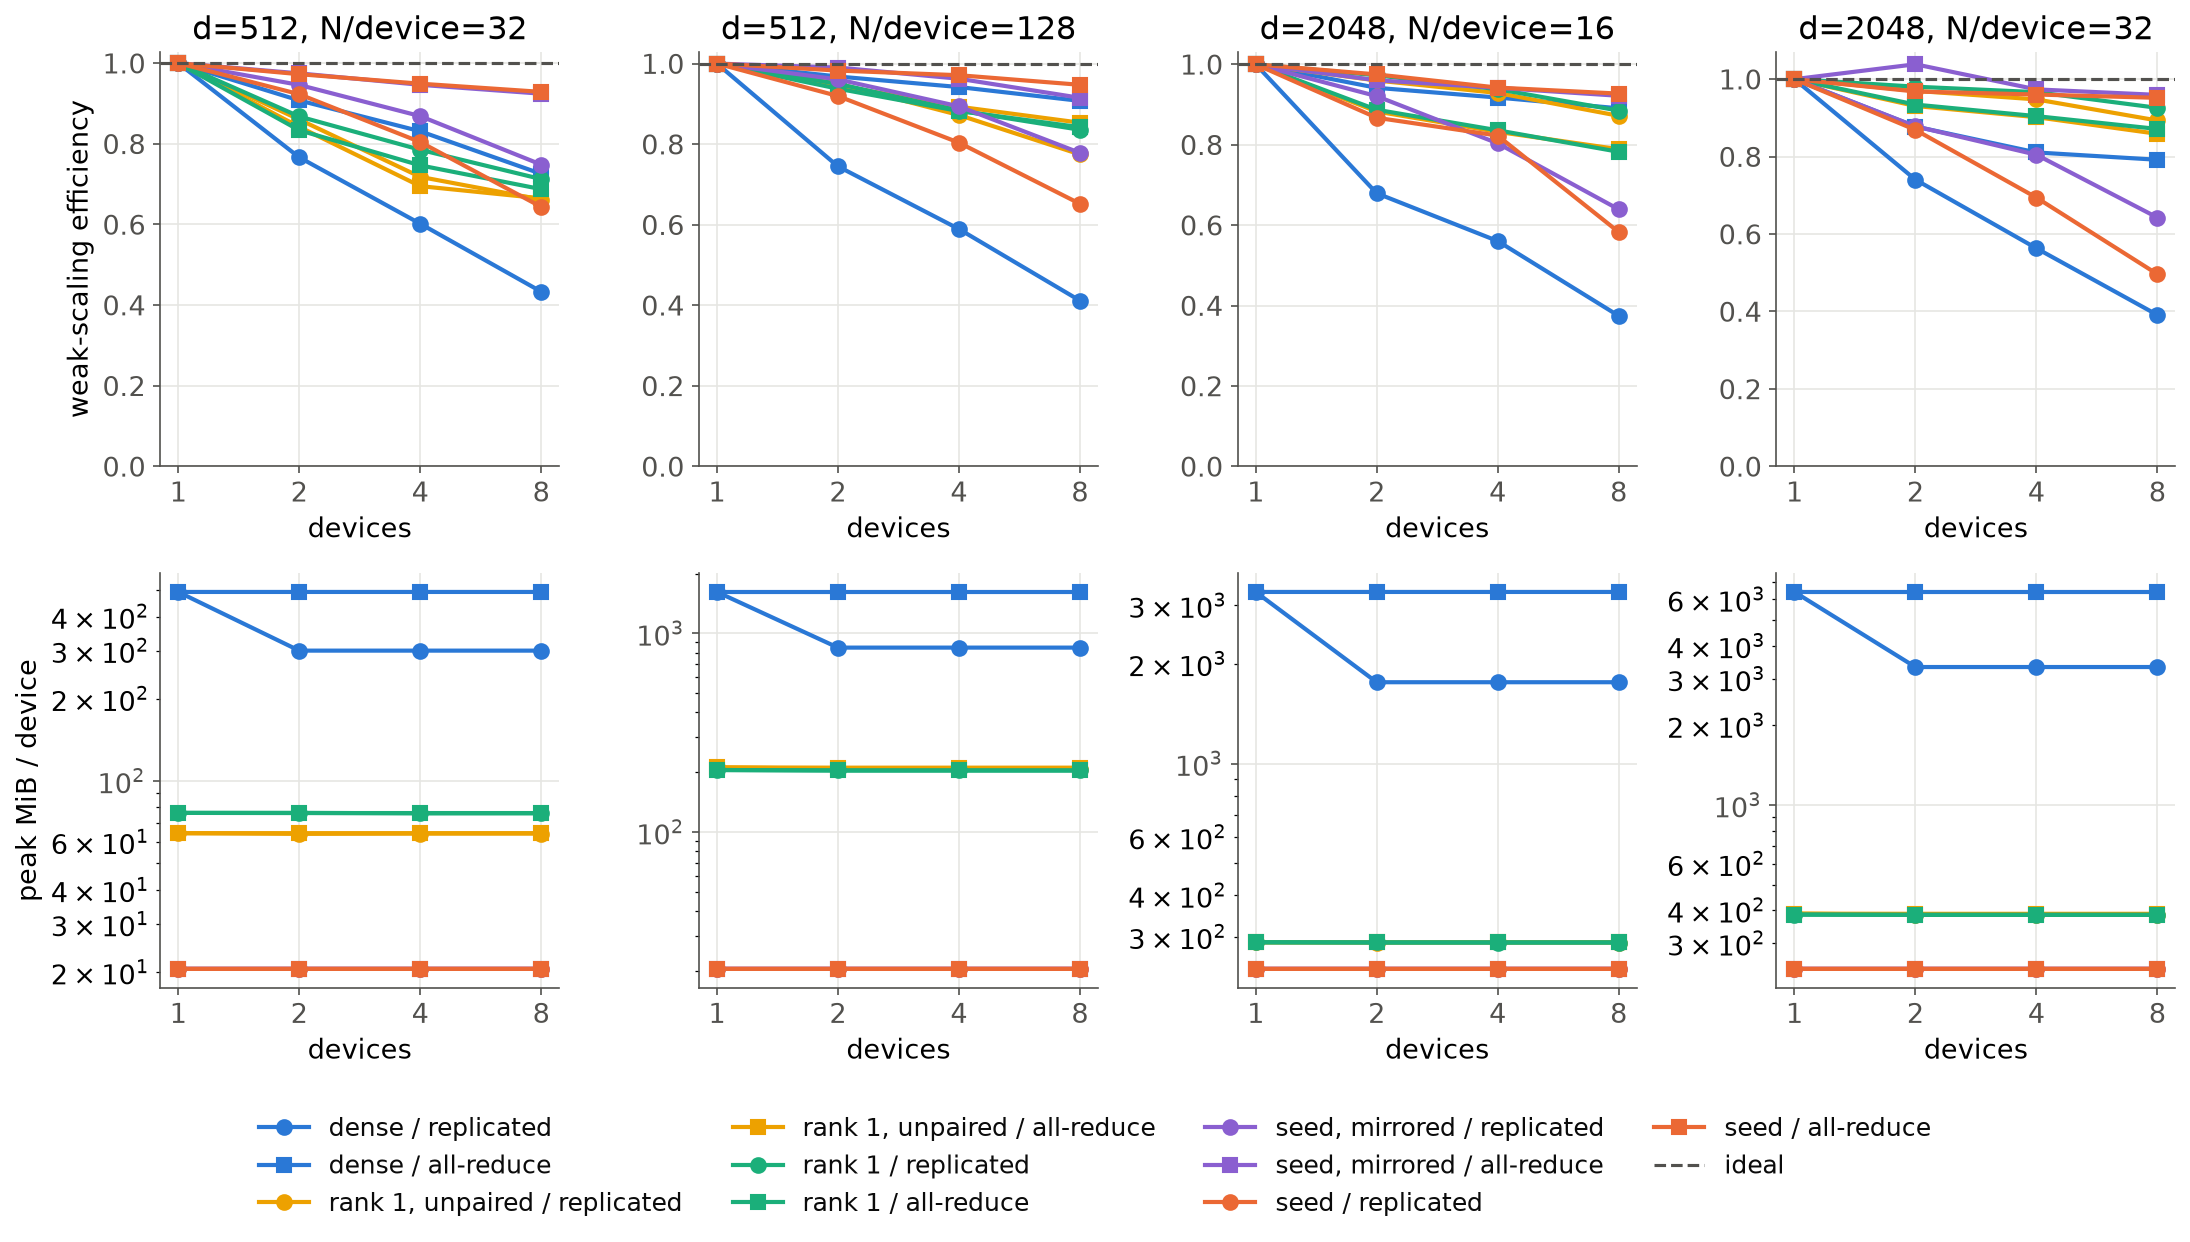
\includegraphics[width=.9\textwidth]{../experiments/phase2/figures/m2-weak-scaling.png}
  \caption{A100 weak scaling: population per device stays fixed. Top: throughput per
    device relative to each series' smallest device count; 1 is ideal. Bottom: peak
    memory per device. A flat memory curve means adding devices does not increase that
    variant's per-device memory requirement at the stated population per device.}
  \label{fig:m2-a100}
\end{figure*}
\begin{figure*}[p]
  \centering
  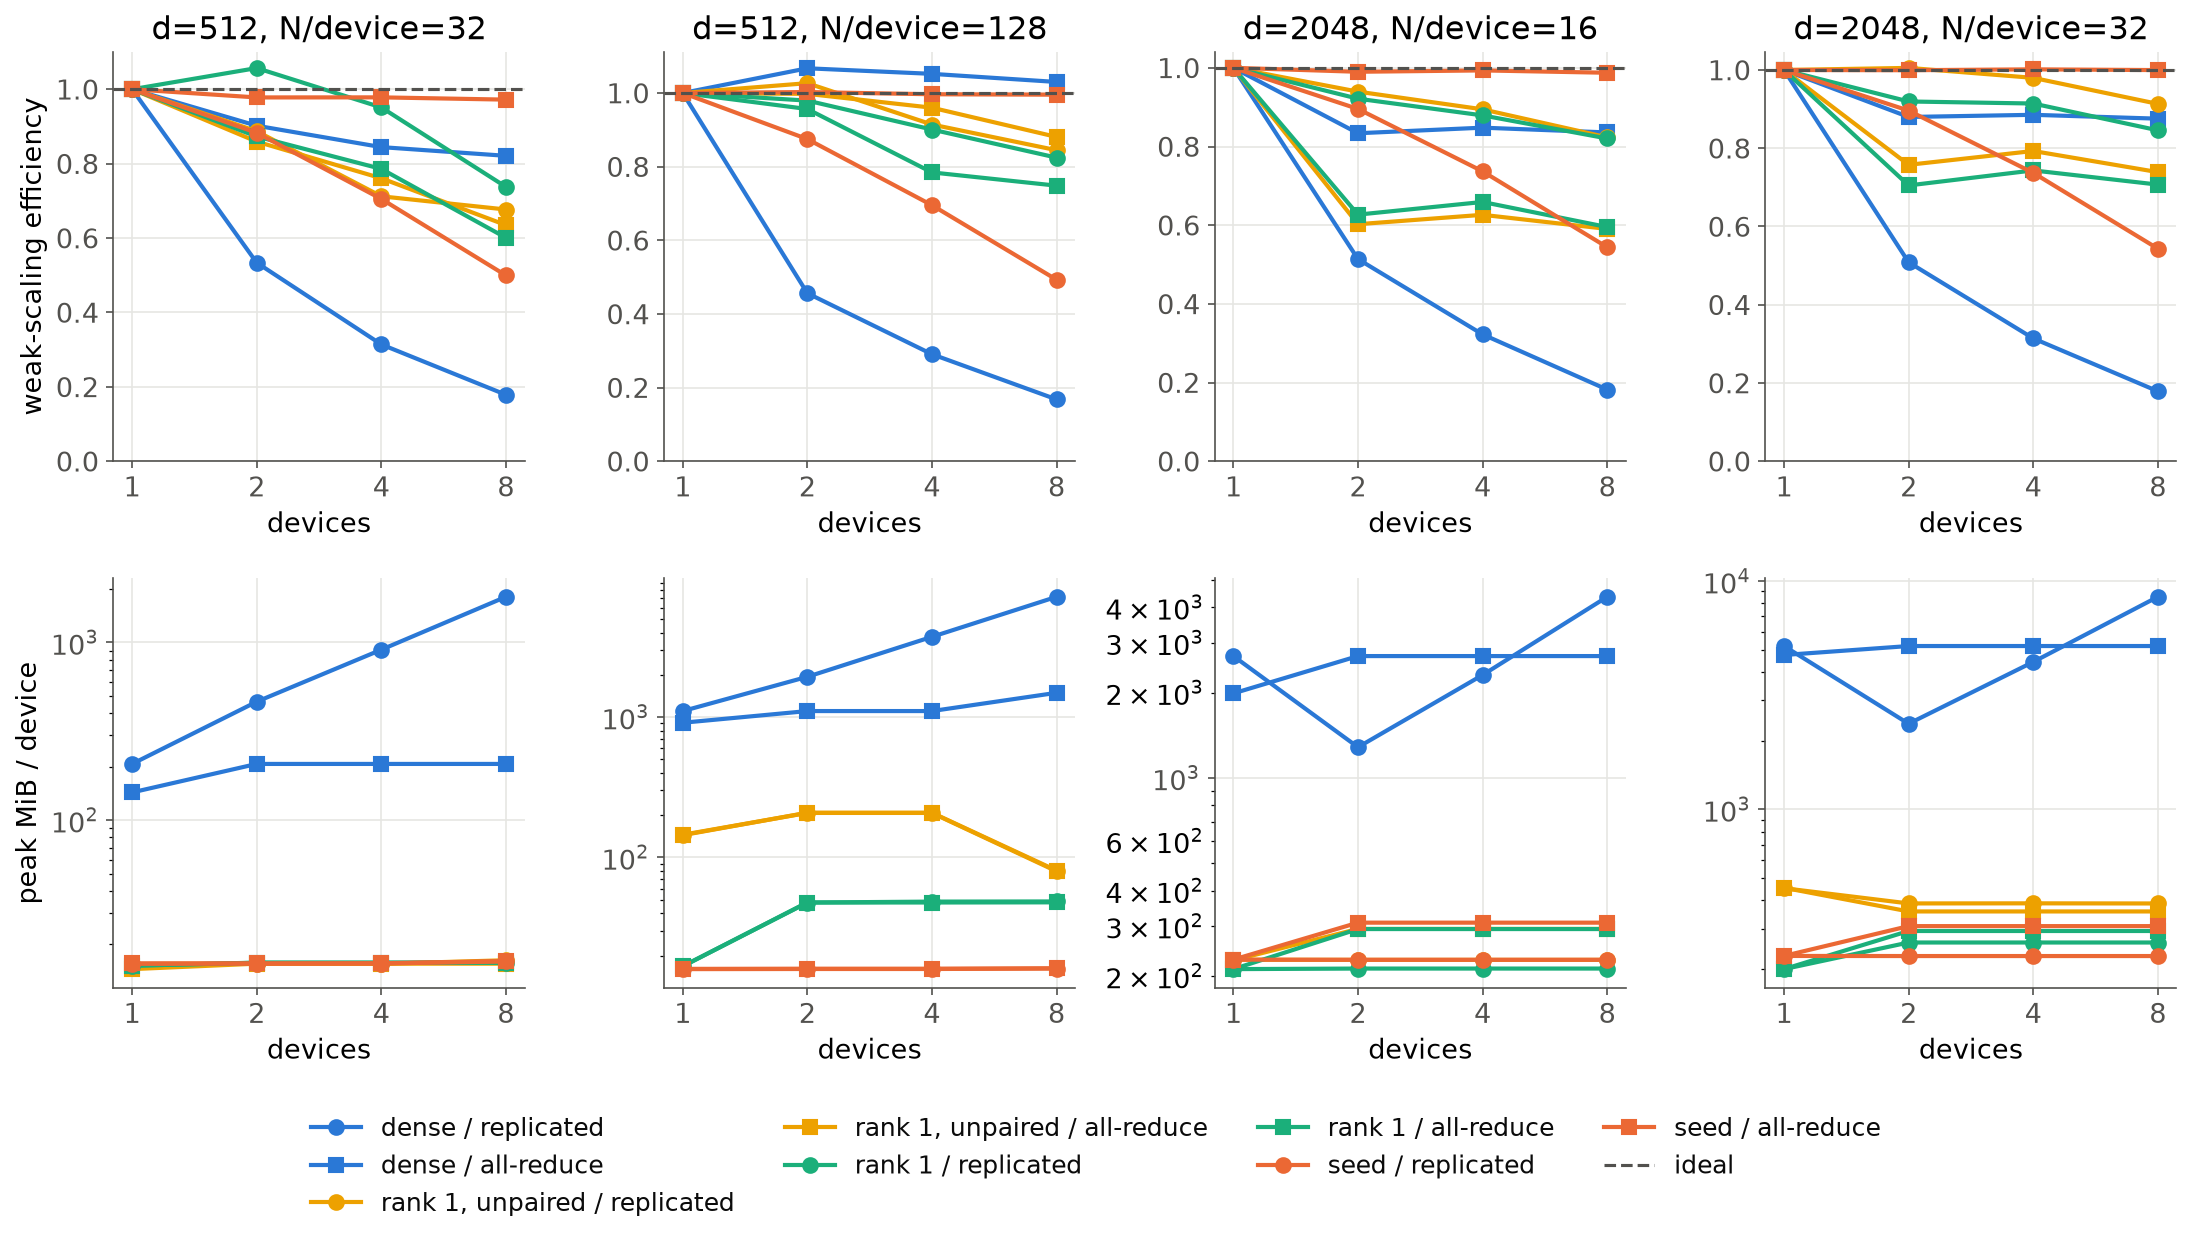
\includegraphics[width=.9\textwidth]{../experiments/phase2/figures-tpu-v5e8/m2-weak-scaling.png}
  \caption{TPU weak scaling at fixed population per device: relative throughput per
    device (top) and peak memory (bottom). Replicated dense reconstruction has the
    largest efficiency loss and its memory grows with the total population.}
  \label{fig:m2-tpu}
\end{figure*}


\section{Reproduction}
\label{sec:repro}

The measurement figures and tables regenerate from scripts and saved results in the
experiments' repository. Each results directory's README records the session that
produced it, including the platform, code version, environment and incidents. The library
is released publicly \librarycite{}; the experiments and manuscript are at \paperurl{}.

In \texttt{experiments/phase2}, \texttt{plot\_paper.py} generates the block-placement
plot, \texttt{plot\_cost.py} the main and appendix cost plots, and \texttt{plot.py}
the scaling grids. In \texttt{experiments/countdown}, \texttt{plot\_e13.py} generates
both the main learning curves and the frozen-embedding comparison;
\texttt{plot\_e19.py} generates the population-16 comparison and \texttt{plot\_e17.py}
the real-model placement plot. The synthetic-alignment plot comes from
\texttt{experiments/phase0/plot.py}.

\texttt{make -C paper} runs the table generators and the revised figure generators,
then builds the PDF. \texttt{paper/Makefile} lists the commands, and
\texttt{paper/README.md} explains how to select the Python environment. Each table
generator accepts \texttt{--latex} and writes the file included in the manuscript;
generated tables are not edited by hand.

The worked example, model comparisons, matched-precision check, bandwidth thresholds
and training displacement ranges are reproduced by \texttt{phase2/paper\_evidence.py}.
The timing ranges are printed by \texttt{phase2/timemodel.py}, the overlap bound by
\texttt{phase2/overlap\_bound.py}, and the compiled-program byte counts by
\texttt{phase2/comms.py} and \texttt{phase2/tb2.py}. The library's device-count
invariance test runs on CPU with eight simulated devices. Continuous integration checks
that regenerating tables changes no bytes and that every commit cited by a result record
remains available.


\end{document}
